{\documentclass[authoryear]{elsarticle}


\makeatletter
\def\ps@pprintTitle{%
\let\@oddhead\@empty
\let\@evenhead\@empty
\def\@oddfoot{}%
\let\@evenfoot\@oddfoot}
\makeatother


\setlength\arraycolsep{2pt}
\setlength{\parskip}{1ex plus 0.5ex minus 0.2ex}
\usepackage{graphicx}
\usepackage{amsfonts}
\usepackage{multirow}
\usepackage{comment}

%\usepackage{chicago}
\bibliographystyle{chicago}





\newcommand{\tr}{\mathrm{tr}}
\newcommand{\e}{\mathrm{e}}
\newcommand{\de}{\mathrm{d}}






%\renewcommand{\labelenumi}{(\roman{enumi})}

\newcommand{\cq}{,\quad }
\newcommand{\qq}{\quad \Rightarrow \quad}

%REFERENCES
\newcommand{\eref}[1]{(\ref{#1})}
\newcommand{\fref}[1]{Figure \ref{#1}}
\newcommand{\sref}[1]{\S\ref{#1}}
\newcommand{\tref}[1]{Table \ref{#1}}
\newcommand{\aref}[1]{\ref{#1}}


%notation for this paper

%EXPECTATIONS AND VARIANCES
\newcommand{\var}{{\rm var}}
\newcommand{\cov}{{\rm cov}}
\newcommand{\cor}{\mathrm{cor}}
\newcommand{\E}{{\mathrm E}}
\newcommand{\p}{{\mathrm P}}
\newcommand{\Ex}{{\mathcal E}}

%DENSITIES
\newcommand{\ft}{{\tilde{f}}}
\newcommand{\Ft}{{\tilde{F}}}




\newcommand{\bi}{\begin{itemize}}
\renewcommand{\i}{\item}
\newcommand{\ei}{\end{itemize}}



\begin{document}


\begin{frontmatter}

\title{Mean and risk densities and their applications to risk management}
\author[acst]{Weihao Choo\corref{cor1}}
\ead{weihao.choo@mq.edu.au}
\author[acst]{Piet de Jong}



\address[acst]{Department of Actuarial Studies Macquarie
University, NSW 2109, Australia.}
\cortext[cor1]{Corresponding author}




\begin{abstract}
This paper proposes a framework to analyze mean and distortion risk across layers forming a random loss. Layers are standard insurance and financial constructs representing insurance coverage, capital shortfall, derivative payouts and debt tranches. Layers are expressed using percentiles or Value-at-Risk which adjust to the shape and scale of the probability distribution. The framework yields insights and solutions to common risk management problems which are difficult or awkward to solve using standard statistical methods.


\end{abstract}

\begin{keyword}
Layers; density; distortion; value-at-risk; reinsurance; tranches.
\end{keyword}



\end{frontmatter}




\section{Introduction to layers and this paper}\label{sintroduction}

This section first summarises the well established concept of layers and their practical applications. Key contributions of this paper are then highlighted and are developed in subsequent sections.

The layer $[a,b]$ of a random loss $x\ge 0$ is defined as the excess of $x$ over $a$ with the excess capped at $b-a$:
$$
\min\{\max(x-a,0),b-a\} = L_b(x)-L_a(x) \cq L_k(x) \equiv \min(x,k)\;,
$$
where $L_k(x)$ is $x$ capped at $k$. Of interest in this paper are layers over various $k$ for a single random variable $x$, thus drop $x$ from the notation and write the layer $[a,b]$ of $x$ as $L_b-L_a$. However keep in mind that layers are functions of $x$ and are hence random variables.


Layers are standard insurance and financial constructs. For example insurance and reinsurance with excess $a$ and limit $b$ cover the layer $[a,b]$ of loss $x$. A capital buffer $k$ divide a loss into two layers -- capital consumed $[0,k]$ and capital shortfall $[k,\infty]$. Derivatives and collaterised debt obligations also involve layers, sometimes known as tranches. For example the payout on a call option on $x$ with exercise price $k$ is the layer $[k,\infty]$, whereas the payout on a put option is $k$ minus the $[0,k]$ layer. A debt may be split into tranches $[a,b]$ where $a$ is the attachment point and $b$ is the detachment point. High layers capture rare, extreme outcomes and low layers characterise common, attritional outcomes.

Statistical properties of layers are discussed in \cite{campana2014risk}, \cite{wang1998actuarial}, \cite{wang1995insurance} and \cite{miccolis1977theory}. \cite{lee1988mathematics} adopts a graphical approach to explain key concepts and results. The insurance pricing of loss layers is discussed in \cite{evans2001exposure} and \cite{salzmann1963rating}. \cite{mandel2012role} and \cite{duffie2001risk} discuss tranches in collaterised debt obligations and how they partially enhance the credit quality of the debt.


The following result is central to this paper:
\begin{equation}\label{layer}
x = L_\infty - L_0 = \int_0^\infty \de L_k = \int_0^\infty L_k' \de k = \int_0^\infty I_k(x) \de k \;,
\end{equation}
where $L_k'$ is the derivative of $L_k$ with respect to $k$ and is equal to
$$
I_k(x) \equiv \left\{\begin{array}{cc}0\ , & x\le k\ ,\\ 1\ ,& x>k\ ,\end{array}\right.
$$
an indicator for $x>k$.

In \eref{layer}, $x$ is composed of infinitesimally small layers $\de L_k$, called the $k$--layer of $x$. The $k$--layer of $x$ is equal to $I_k(x) \de k$, an increment $\de k$ if $x$ exceeds $k$. Each $k$--layer is a random variable and is comonotonic with all other layers since $\de L_k$ is non-decreasing in $x$. The layer decomposition of $x$ in \eref{layer} is key to analyzing sources of mean and risk in a loss as shown subsequently in this paper.

Integrating $k$--layers from $a$ to $b$ reproduces the $[a,b]$ layer:
$$
\int_a^b \de L_k = L_b-L_a = \min(x,b)-\min(x,a) = \min\{ \max(x-a,0) ,b-a\} \;.
$$

Assuming $x$ has distribution function $F$, the mean of layer $\de L_k $ is
$$
\E(\de L_k) = \E\left\{I_k(x)\de k\right\}=\{1-F(k)\} \de k
$$
where $\E$ is the expectation. \cite{wang1996pct} calls $1-F$ the layer premium density of $x$ as it indicates the mean value or insurance premium of each layer and it integrates to the overall premium: $\int_0^\infty \{1-F(k) \}\de k = \E(x)$. \cite{wang1996pct} also distorts $1-F$ to deliver risk-adjusted premiums.


This paper modifies and extends results in \cite{wang1996pct} by defining ``VaR layers": layers expressed on the percentile or Value-at-Risk (VaR) scale. VaRs adjust to the shape and scale of the loss distribution, and are hence comparable across loss distributions. VaRs are standard insurance and financial constructs. For example Solvency II insurance regulation applies $90\%$ and $99.5\%$ VaRs \citep{eling2007solvency} to capital requirements. Banking regulations Basel II and Basel III also reference VaRs in risk measurement \citep{chernobai2008operational}.



A framework is constructed to analyse mean and distortion risk across VaR layers forming a random loss. The framework yields insights and solutions to risk management problems such as setting optimal capital buffers, analyzing the credit quality of debt tranches, and applying reinsurance to transform the loss distribution. These problems are typically difficult or awkward to express and solve using standard statistical approaches. In addition optimal quantities derived from the framework, such as capital buffers, are expressed in VaRs which are standard references in finance and insurance as mentioned above.


Remaining sections of this paper are structured as follows. VaR layers are first defined in section \aref{ssetup}. Sections \aref{smean} to \aref{sprop} formalise, analyze and illustrate layer means or ``mean densities." Risk densities are covered in sections \aref{srisksetup} to \aref{sproprisk}. Section \aref{sempirical} shows how mean and risk densities are calculated from data and illustrates using historical stock returns. Remaining sections apply mean and risk densities to insurance pricing, collaterised debt obligations, capital setting and reinsurance loss transformation.


\begin{comment}

\section{Motivating example}\label{smotivating}

Whilst \eref{layers} provides the key initial mathematical result, the following example provides further motivation for developments in this paper.

Consider $100$ ordered observations of an insurance loss $x$: $x_1<x_2<\ldots<x_{100}$. The statistics $x_{i+1}-x_i$ and $(100-i)(x_{i+1}-x_i)$ are called the spacing and normalised spacing, respectively, in the order statistics \citep{shaked2007stochastic}. Spacings are of interest in engineering, for example corresponding to elapsed times between successive  failures of components forming a system.

Spacings define layers of an insurance loss. In terms of spacings, the sample mean of  $x$ is
\begin{equation}\label{mean}
\bar{x}=   x_1 + \frac{99}{100} (x_2-x_1) +\ldots + \frac{100-i}{100} (x_{i+1}-x_i)+\ldots +\frac{1}{100}(x_{100}-x_{99})  \;,
\end{equation}
of which the mean contribution of layer $[x_i,x_{i+1}]$ given the sample is
$$
m_i \equiv \left(\frac{100-i}{100}\right) (x_{i+1}-x_i)\ ,
$$
then  $m_i$ is the spacing $x_{i+1}-x_i$ multiplied by the proportion or probability  $1-i/100$ of an observation exceeding $x_i$.  Adding up all $m_i$  yields the overall mean $\bar{x}$.  A layer is a portion of every loss outcome crossing an interval.

The following are important and exploitable points of the above setup:
\bi

\i Two  factors drive the magnitude  of $m_i$:   the exceedance  probability   $1-i/100$ and spacing $x_{i+1}-x_i$.  The exceedance probability decreases  with $i$.   The spacing may increase or decrease.   If the distribution is right skewed, as is typical for insurance losses, increasing $i$, leads to increased spacings.   Greater skewness implies larger spacings.    The overall behaviour of $m_i$ characterises the shape of the loss distribution.

\i Loss layers are expressed using sample values representing empirical percentiles or values-at-risk (VaRs) of $x$. For example the top 5 loss layer covers losses above the $95$th percentile. In contrast, current literature expresses loss layers in absolute amounts, for example between 1 and 2 million dollars. VaR layers are considered in this paper as they adjust to the shape and scale of the loss distribution, and can be interpreted probabilistically.

\i Individual layer means $m_i$ are building blocks for assessing expected coverage and related quantities. For example $m_1+m_2+\ldots+ m_{75}$ is the mean insured loss if coverage is limited to the 75th percentile. The sum $m_{95}+m_{96}+m_{97}+m_{98}+m_{99}$ is the mean of excess losses above the $95$th percentile, and represents the expected shortfall if capital is held at the $95$th percentile, or the expected excess-of-loss reinsurance coverage above the $95$th percentile.


\i The risk-adjusted layer mean replaces the exceedance probability $1-i/100$ in $m_i$ with a distorted probability $1-\Phi(i/100)$, yielding
$$
\tilde{m}_i = \left\{1-\Phi\left(\frac{i}{100}\right)\right\} (x_{i+1}-x_i)\ .
$$
Distorted probabilities shape layer means, yield distorted risk measures \citep{wang1996pct}  and are used in cumulative prospect theory \citep{tversky1992apt}.

\ei

\end{comment}



\section{Decomposing a loss into VaR layers}\label{ssetup}


Consider a continuous random loss $x\geq 0$ with distribution function $F$ and inverse distribution function $F^-$. For any constant $0\le\alpha\le 1$, the $\alpha$--VaR or VaR$_\alpha$ of $x$ is  $V_\alpha\equiv F^-(\alpha)$. Substituting $k=V_\alpha$ into \eref{layer} yields
$$
x=L^*_1-L^*_0=\int_0^1 \de L^*_\alpha = \int_0^1  (L^{*}_\alpha)'  \de \alpha = \int_0^1 I_{V_\alpha}(x) V_\alpha' \de \alpha  \;,
$$
where $V_\alpha'$ is the derivative of $V_\alpha$ with respect to $\alpha$ and $L_\alpha^*\equiv L_{V_\alpha}=\min(x,V_\alpha)$ is the capped loss with the cap expressed in VaRs instead of dollars. VaRs are used for the rest of this paper, hence drop the superscript $^*$ in the notation. In addition define $u\equiv F(x)$ as the percentile rank of $x$ and hence $I_{V_\alpha}(x)=I_\alpha(u)$.

Therefore rewrite the above result using the simplified notation
\begin{equation}\label{varlayer}
x=L_1-L_0=\int_0^1 \de L_\alpha = \int_0^1  L'_\alpha  \de \alpha = \int_0^1 I_\alpha(u) V_\alpha' \de \alpha  \;.
\end{equation}
Similar to \eref{layer}, \eref{varlayer} decomposes $x$ into infinitesimally small VaR layers. The $V_\alpha$--layer of $x$ is $\de L_\alpha=I_\alpha(u) V_\alpha' \de \alpha$, an increment $V_\alpha' \de\alpha$ if $x>V_\alpha$ or $u>\alpha$. The increment is proportional to $V_\alpha'$ called the $V_\alpha$--spacing, analogous to spacings between order statistics \citep{shaked2007stochastic}. VaR spacings vary across a loss distribution with larger spacings indicating areas of greater skewness. Increasing the scale of a loss distribution increases VaR spacings by the same scale. The $V_\alpha$--spacing can be written as
$$
V_\alpha' = \frac{\de}{\de\alpha} F^-(\alpha) =  \frac{1}{f(V_\alpha)} \cq f\equiv F'
$$
where $f$ is the loss density. Hence $V_\alpha$--spacing is increasing in the upper tail of a right skewed distribution where the density gradually tails off to 0.

Similar to \sref{sintroduction}, integrating $V_\alpha$--layers forms a larger VaR--layer:
$$
\int_\alpha^\beta \de L_\pi = L_\beta-L_\alpha = \min(V_\beta,x)-\min(V_\alpha,x) = \min\{\max(x-V_\alpha,0),V_\beta-V_\alpha\}
$$
the excess of $x$ over $V_\alpha$ with the excess capped at $V_\beta-V_\alpha$. The VaR--layer $[V_\alpha,V_\beta]$ is positive when $u>\alpha$, with probability $1-\alpha$, and reaches its maximum $V_\beta-V_\alpha$ when $u>\beta$, with probability $1-\beta$.

Hence a VaR--layer captures a portion of losses identified from their relative position in the probability distribution. For example the VaR--layer $[V_{0.5},V_{0.75}]$ captures the top $50\%$ of losses, and the top $25\%$ of losses are capped at the 75th percentile. Endpoints of VaR layers self-adjust to the shape and scale of the loss distribution. Increasing the scale of the loss distribution increases layer endpoints by the same scale, and similarly when skewness increases. VaR layers are therefore comparable between loss distributions with different scale or shape. In contrast layers determined in dollar terms as in \sref{sintroduction} may be attritional or extreme layers depending on the loss distribution.



\section{Mean density -- expected values of VaR layers}\label{smean}


Following \cite{wang1996pct}, define the mean density of $x$ as the relative mean value of the $V_\alpha$--layer, yielding
\begin{equation}\label{meancont}
m_\alpha \equiv \E(L'_\alpha)=\E\left\{I_\alpha(u)V_\alpha' \right\}
=(1-\alpha)V_\alpha'   \;,
\end{equation}
for $0\le\alpha\le 1$. The mean density $m_\alpha$ is the product of $1-\alpha$, the probability of $x$ reaching $V_\alpha$, and the $V_\alpha$--spacing $V_\alpha'$, the width of the $V_\alpha$--layer of $x$.

The behaviour of $m_\alpha$ with $\alpha$ depends on relative movements in $1-\alpha$ and $V_\alpha'$, and characterises the loss distribution as illustrated in \sref{smeaneg}. As $\alpha$ increases, $1-\alpha$ decreases due to a reduced likelihood of $x$ reaching larger VaRs. On the other hand for a right skewed loss distribution where the probability density is decreasing, $V_\alpha'=1/f(V_\alpha)$ increases in $\alpha$.


The term ``density" is used to refer to $m_\alpha$ due to analogous properties shared with probability densities. Using \eref{varlayer},
$$
\int_0^1 m_\alpha \de \alpha = \E\left( \int_0^1 \de L_\alpha \right) = \E(x) \;,
$$
thus the total area under the mean density is the overall mean loss. The mean density hence spreads the overall mean across layers forming the loss, and identifies layers with high mean contribution. Integrating the mean density over the interval $[\alpha,\beta]$ yields the mean of the $[V_\alpha,V_\beta]$ VaR--layer:
\begin{equation}\label{subset}
\int_\alpha^\beta m_\pi\de \pi=\E\left( \int_\alpha^\beta \de L_\pi \right)=\E(L_\beta-L_\alpha)  \;.
\end{equation}
Analogously, integrating a probability density over its entire support yields total probability $1$, whilst integrating over other intervals yields the probability over the same interval.

Mean values of VaR--layers represent, for example, the pure premium under an excess-of-loss reinsurance arrangement, expected capital shortfall or consumed, and expected derivative payouts. Section \aref{srisksetup} defines risk values of VaR--layers. Combining mean and risk values of VaR--layers yields insights to common risk management problems discussed further in \sref{sapplication}.



\section{Example mean densities}\label{smeaneg}


The following are mean densities for common probability distributions. In all cases $b>0$ is a scale parameter.
\bi
\i The  uniform distribution over $[0,b]$ yields
$$
V_\alpha=b\alpha \cq V_\alpha'=b \cq m_\alpha=(1-\alpha)b \;,
$$
hence the mean density linearly decreases to zero. The mean density is decreasing since uniform VaR--spacings are offset by the lower likelihood of losses reaching higher VaRs. The mean density is also proportional to scale $b$, and this is the case for all mean densities described below.


\i The  exponential distribution  with mean $b$ yields
$$
F(x)=1-\e^{-x/b} \cq V_\alpha=-b \ln(1-\alpha) \cq V_\alpha'=\frac{b}{1-\alpha} \cq m_\alpha=b\;,
$$
and the mean density is constant since increasing VaR--spacings exactly offset decreasing probabilities of losses reaching larger VaRs. Hence VaR layers of an exponential distribution have uniform contribution to the overall mean.


\i The  Pareto distribution with shape parameter $c>1$ yields
$$
F(x)=1- \left(\frac{b}{b+x}\right)^c \cq V_\alpha= b\left\{(1-\alpha)^{-1/c}-1\right\} \;,
$$
$$
 V_\alpha'=\frac{b}{c (1-\alpha)^{1/(c+1)}} \cq m_\alpha = \frac{b}{c(1-\alpha)^{1/c}} \;.
$$
The mean density increases to infinity as $\alpha\rightarrow 1$:  increasing VaR spacings more than offset decreasing probabilities of reaching larger VaRs. Mean contributions are concentrated in high VaR layers of a Pareto distribution.

\i For the Weibull distribution with shape parameter $k>0$,
$$
F(x)=1-\e^{-(x/b)^k} \cq V_\alpha = b\left\{- \ln(1-\alpha)\right\}^{1/k} \;,
$$
$$
V_\alpha'=\frac{b\left\{-\ln(1-\alpha)\right\}^{1/(k-1)}}{k(1-\alpha)}  \cq
m_\alpha=\frac{b\left\{-\ln(1-\alpha)\right\}^{1/(k-1)}}{k} \;.
$$
Setting $k=1$ yields the exponential distribution and $m_\alpha=b$. Reducing $k$ increases skewness and yields increasing $m_\alpha$. Vice versa if $k>1$.


\ei
\fref{fmeancont} plots mean densities for the above loss distributions with parameters selected to satisfy $\E(x)=1$. Hence mean densities in \fref{fmeancont} all integrate to one, and their shape indicates relative contributions from different layers of the loss. As described above, the exponential distribution has a flat mean density and the overall mean value is spread uniformly across VaR layers. For the Pareto distribution, the bulk of the overall mean value is contributed by high VaR layers as reflected by an increasing mean density. The opposite applies to the uniform distribution and the Weibull distribution ($k>1$ in this case).
\begin{figure}
  \begin{center}
    \begin{tabular}{cc}
      \resizebox{120mm}{!}{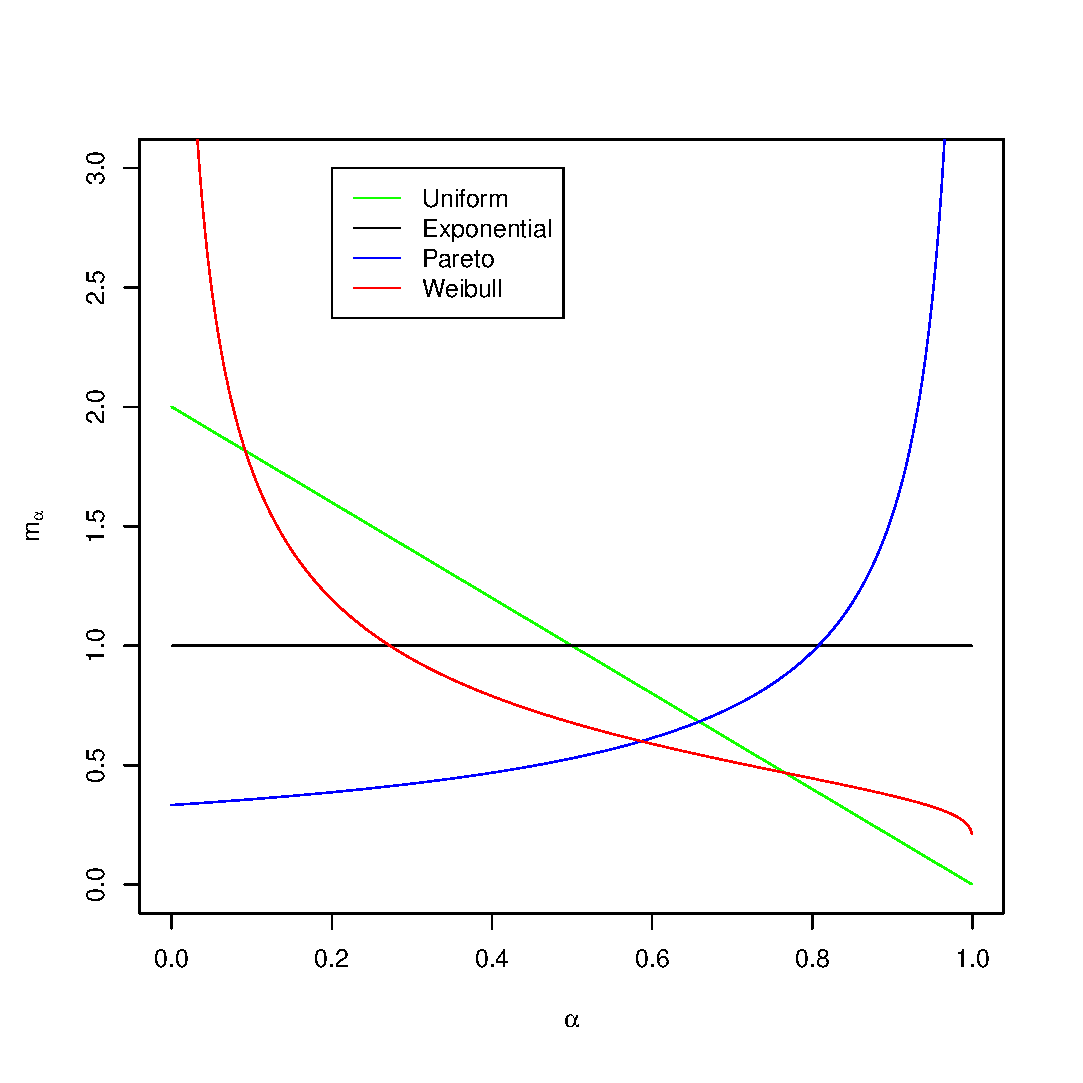
\includegraphics{meancont.eps}}
    \end{tabular}
    \caption{Mean densities for uniform ($b=2$), exponential ($b=1$), Pareto ($b=0.5$, $c=1.5$) and Weibull ($b=1.13$, $k=2$) distributions. All distributions have mean 1 hence the area underneath each curve is 1.}
    \label{fmeancont}
  \end{center}
\end{figure}

The constant mean density for the exponential distribution provides a benchmark for assessing skewness at various parts of a loss distribution. A decreasing mean density (for example uniform distribution and Weibull distribution for $k>1$) implies VaR--spacings increase at a lower rate compared to the exponential, and hence lower skewness comparatively. Vice versa for an increasing mean density (for example Pareto distribution and Weibull distribution for $k<1$). The derivative of $m_\alpha$ with respect to $\alpha$ is
$$
m'_\alpha=(1-\alpha)V_\alpha''-V_\alpha' \;.
$$
Hence the mean density is increasing at $\alpha$ if and only if $(1-\alpha)V_\alpha''/V_\alpha'>1$. Rewriting this inequality in terms of the loss density $f$ yields the condition
$$
\frac{(1-\alpha)V_\alpha''}{V_\alpha'} = -\frac{(1-\alpha)f'(V_\alpha)}{\{f(V_\alpha)\}^2} > 1
\cq
V_\alpha''= - \frac{f'(V_\alpha)}{\{f(V_\alpha)\}^3}
$$
The probability distribution of $x$ has greater skewness than the exponential over layers where the above inequality holds, and vice versa.



\section{Properties of mean densities}\label{sprop}


\subsection{Monotonic loss transformations}

Straightforward changes apply to the mean density when a monotonic transformation is applied to the loss. Consider the transformation $y=g(x)$ where $g>0$ is an increasing function. Then $y$ has VaR$_\alpha$ $V_\alpha(y)=g\{V_\alpha(x)\}$ and the mean density of $y$ at the VaR$_\alpha$ layer is
$$
m_\alpha(y) = (1-\alpha)V'_\alpha(y) = (1-\alpha)g'\{V_\alpha(x)\}V_\alpha'(x)=m_\alpha(x) g'\{V_\alpha(x)\} \;,
$$
where $V_\alpha(x)$ and $m_\alpha(x)$ are respectively the VaR$_\alpha$ and mean density of $x$. Hence the mean density of $y$ is the mean density of $x$ multiplied by the derivative $g'\{V_\alpha(x)\}$. In particular if $y=cx$ where $c$ is constant then $m_\alpha(y)=cm_\alpha(x)$. This result implies mean densities are proportional to the scale of the loss distribution, as demonstrated by the examples in \sref{smeaneg}.

It is also straightforward to show that if $y=g(x)$ is a decreasing transformation then $V_\alpha(y)=g\{V_{1-\alpha}(x)\}$ and $m_\alpha(y)=m_{1-\alpha}(x)g'\{V_{1-\alpha}(x)\}$. Hence in this case the mean density of $x$ at the $V_{1-\alpha}$--layer is referenced.


\subsection{Unique characterisation of the loss distribution}

Assuming $V_0=0$, the mean density uniquely characterises the loss distribution. Re-arranging \eref{meancont} and integrating yields
$$
F^-(\alpha) = V_\alpha = \int_0^\alpha \frac{m_\pi}{1-\pi} \de \pi  \;.
$$
VaR$_\alpha$ is a weighted cumulative of the mean density up to the VaR$_\alpha$ layer. Larger mean density values lead to greater VaRs.


\subsection{Connection to hazard function}


Substituting $V'_\alpha=1/f(V_\alpha)$ to \eref{meancont} yields
$$
m_\alpha =  \frac{1-\alpha}{f(V_\alpha)}  = \left\{\frac{f(V_\alpha)}{1-F(V_\alpha)}\right\}^{-1}  \cq F(V_\alpha)=\alpha \;.
$$
Therefore the mean density at the $V_\alpha$--layer of $x$ is the reciprocal of the hazard function \citep{hogg2009loss} at $x=V_\alpha$. The hazard at $V_\alpha$ indicates the instantaneous probability of $x=V_\alpha$ given it reaches $V_\alpha$. The above result implies a lower hazard at $V_\alpha$ leads to a higher mean value of the $V_\alpha$--layer.





\section{Risk density -- distortion risks of VaR layers}\label{srisksetup}


This section defines risk densities which indicate the distortion risk of VaR layers. Similar to mean densities, risk densities identify contributions by various VaR layers to overall risk. Risks are important inputs to decisions involving volatility. For example premium loadings, capital buffers and expected investment returns are driven by risk values. Mean values are insufficient decision making inputs as they do not capture the spread of outcomes.

\cite{wang1996pct} defines distortion risk based on the mean value under a distorted distribution function $\Phi\circ F$ where $\Phi$ is an increasing, convex distortion operator satisfying $\Phi(0)=0$ and $\Phi(1)=1$. The distortion risk of $x$ is hence
$$
r\equiv \Ex(x) - \E(x) = \int_0^\infty \left[ 1-\Phi\{F(x)\} \right] \de x - \int_0^\infty \{ 1-F(x)\} \de x  \;,
$$
where $\Ex$ calculates expectations under the distorted distribution $\Phi\circ F$. \cite{choo2009loss} shows the equivalence between distortion risks, loss aversion premiums and spectral risks \citep{acerbi2002spectral}. Examples of distortion risks using various $\Phi$ are discussed in \cite{wang1995insurance}, \cite{wang2000cdo} and \cite{choo2009loss}, and include the proportional hazards risk, conditional-tail-expectation and expected-maximal-loss. Distortion risks are coherent \citep{artzner1999cmr}: positively homogenous, translation invariant, monotonic and subadditive.

The risk density of $x$ indicates the distortion risk of the $V_\alpha$--layer of $x$ and applying similar calculations as above yields
\begin{equation}\label{riskcont}
r_\alpha \equiv \Ex(L'_\alpha)-\E(L'_\alpha) =
\{1-\Phi(\alpha)\}V_\alpha'-(1-\alpha)V_\alpha'=\{\alpha-\Phi(\alpha)\}V_\alpha'\ .
\end{equation}
This result follows since $\Ex\{I_\alpha(u)\}$ is the distorted probability of $u>\alpha$ which is $1-\Phi(\alpha)$, whereas the original probability is $1-\alpha$. Note $r_\alpha\geq 0$ for all $\alpha$ since $\Phi$ is convex implying $\Phi(\alpha)\le\alpha$.

The risk density $r_\alpha$ in \eref{riskcont} is composed of two factors. The difference $\alpha-\Phi(\alpha)$ represents the extent of distortion at $V_\alpha$, with $\alpha=\Phi(\alpha)$ indicating zero distortion and $r_\alpha=0$. The other factor is layer width or $V_\alpha$--spacing $V_\alpha'$. Increasing either factor increases $r_\alpha$.


Similar to mean densities, integrating risk densities yields the risk of larger VaR layers. Integrating $r_\alpha$ over all $\alpha$ yields the overall distorted risk of $x$:
$$
\int_0^1 r_\alpha \de \alpha = \int_0^1 \{\Ex(L'_\alpha)-\E(L'_\alpha)\} \de \alpha = \Ex(x)-\E(x) = r\;.
$$
Alternatively, $V_\alpha$--layers over all $0\le\alpha\le 1$ are comonotonic, and distortion risks of comonotonic random variables are additive \citep{wang1997aci}. Integrating $r_\alpha$ over $[\alpha,\beta]$ yields the distorted risk of VaR--layer $[V_\alpha,V_\beta]$:
$$
\int_\alpha^\beta r_\pi \de \pi = \Ex\left(L_\alpha-L_\beta\right)-\E\left(L_\alpha-L_\beta\right)  \;.
$$
Again an analogous property applies to probability densities.



\begin{comment}
The end points of VaR layers are unchanged at $V_\alpha=F^-(\alpha)$, even though the $\mathrm{VaR}_\alpha$ of the distorted distribution is $F^-\{\Phi^-(\alpha)\}$. Therefore end points of VaR layers are fixed and specified using the original distribution, and distortion only affects the probability distribution of a layer.


The above integral represents for example the risk loading on the premium for an insured or reinsured loss, and the risk of the capital shortfall amount. These are important inputs to pricing, capital and other risk management decisions. The risk density spreads the overall risk of a random loss across its VaR layers, and generally more focus is placed on managing layers with higher risk. Applications of mean and risk densities are discussed in \sref{sapplication}.



\end{comment}




\section{VaR risk ratios}


The risk ratio at the $V_\alpha$--layer is the ratio between risk and mean densities:
\begin{equation}\label{riskratio}
r_\alpha^* \equiv \frac{r_\alpha}{m_\alpha} = \frac{\{\alpha-\Phi(\alpha)\}V_\alpha'}{(1-\alpha)V_\alpha'} = \frac{\alpha-\Phi(\alpha)}{1-\alpha} \;,
\end{equation}
noting $V_\alpha'$ appears in both numerator and denominator and hence cancels after division. Risk ratios indicate the risk of a VaR--layer relative to its mean. Risk ratios only depend on the distortion operator $\Phi$ and are independent of the loss distribution. Risk ratios are also larger at higher layers, since
$$
\frac{\de r_\alpha^*}{\de \alpha} = \frac{1-\Phi(\alpha)-(1-\alpha)\Phi'(\alpha)}{(1-\alpha)^2} \geq 0 \;.
$$
The inequality holds since
$$1-\Phi(\alpha)=\int_\alpha^1 \Phi'(u) \de u\geq \int_\alpha^1 \Phi'(\alpha)\de u=(1-\alpha)\Phi'(\alpha)\ ,
$$
noting $\Phi$ is convex hence $\Phi'$ is increasing. Thus higher VaR--layers are always relatively riskier than lower VaR--layers as a proportion of their mean value. Risk ratios at the lowest and highest VaR--layers are $r_0^* = 0$ and $r_1^*=\Phi'(1)-1$ respectively, where the latter is derived using the  L'H\^{o}pital's rule.



The overall risk ratio of $x$ can be written in terms of $r_\alpha^*$ as
$$
\frac{r}{\E(x)} = \frac{\int_0^1 r_\pi \de \pi}{\int_0^1  m_\pi \de \pi}
=\frac{\int_0^1 r_\pi^* m_\pi \de \pi}{\int_0^1  m_\pi \de \pi}    \; .
$$
Therefore the overall risk ratio is a weighted average of individual risk ratios. Weights are given by mean density values. As $r_\alpha^*$ is increasing in $\alpha$ and independent of the loss distribution as mentioned above, the overall risk ratio is high if the mean density is high at higher layers resulting in higher risk ratios being weighted more heavily. Hence skewed loss distributions are relatively riskier, consistent with intuition. Using the example mean densities in \sref{smeaneg}, the Pareto has a higher overall risk ratio than the uniform, exponential and Weibull due to an increasing mean density. Examples are further discussed in the next section.





\section{Example risk ratios and risk densities}\label{sriskeg}

The following are risk ratios based on distortion operators discussed in \cite{wang1995insurance} and \cite{choo2009loss}. As highlighted in the previous section, risk ratios only depend on the distortion operator. Multiplying risk ratios with the mean density yields the risk density.

\bi

\i Assume  $\Phi(\alpha)=I_c(\alpha)(\alpha-c)/(1-c)$ where $0\leq c\leq 1$ is a parameter. The overall distortion risk of $x$ involves the conditional-tail-expectation and is given by $\E(x|x>V_c)-\E(x)$, the expected value of losses above $V_c$ in excess of the overall mean loss. The risk ratio using \eref{riskratio} is
$$
r_\alpha^*= \left\{1-I_c(\alpha)\right\} \frac{\alpha}{1-\alpha}+ I_c(\alpha) \frac{c}{1-c} \;.
$$
Risk ratios increase from 0 at the lowest layer and reaches $c/(1-c)$ at the $V_c$--layer, and remains constant at $c/(1-c)$ for higher layers. Note larger $c$ yields higher $r_\alpha^*$ for all $0\le\alpha\le1$, hence  $c$ indicates overall risk aversion.



\i Assume the power distortion operator $\Phi(\alpha)=\alpha^n$ where $n\geq 1$. If $n$ is an integer, the distortion risk is $\E\{\max(x_1,\ldots,x_n)\}-\E(x)$ or the expected-maximal-loss in excess of the mean loss, where $x_1,\ldots x_n$ are independent copies of $x$. The risk ratio in this case is
$$
r^*_\alpha =  \frac{\alpha -\alpha^n}{1-\alpha} =  \sum_{i=1}^{n-1} \alpha^i \;,
$$
where the final expression assumes integer $n$, and is a polynomial of degree $n-1$ with unit coefficients. Larger $n$ yields higher risk ratios for all $\alpha$, hence $n$ indicates risk aversion.


\i Assume the proportional hazards transform, $\Phi(\alpha)=1-(1-\alpha)^{1/\gamma}$ where $\gamma\geq 1$. The distortion risk is $\int_0^\infty \{S(x)\}^{1/\gamma} \de x-\int_0^\infty S(x) \de x$ where $S$ is the survival function, that is $S\equiv 1-F$. The risk ratio is
$$
r_\alpha^*=\frac{\alpha-\{1-(1-v)^{1/\gamma}\}}{1-\alpha} = (1-\alpha)^{1/\gamma-1}-1 \;,
$$
and increases to $\infty$ as $\alpha$ approaches 1. Higher $\gamma$ increases risk ratios across all layers and indicates overall risk aversion.

\ei
The four panels in \fref{frisk} graph mean densities shown in \fref{fmeancont} and risk densities using a power distortion operator $\Phi(\alpha)=\alpha^3$. The risk ratio is $r_\alpha^*=\alpha(1+\alpha)$. For the uniform loss distribution, risk is highest around median VaR--layers since increasing risk ratios are applied to a decreasing mean density. Risk densities are increasing for exponential, Pareto and Weibull loss distributions. Pareto has the highest overall risk (the area under the risk density), since higher risk ratios are applied to higher mean densities at higher VaR layers.

\begin{figure}
  \begin{center}
    \begin{tabular}{cc}
      \resizebox{60mm}{!}{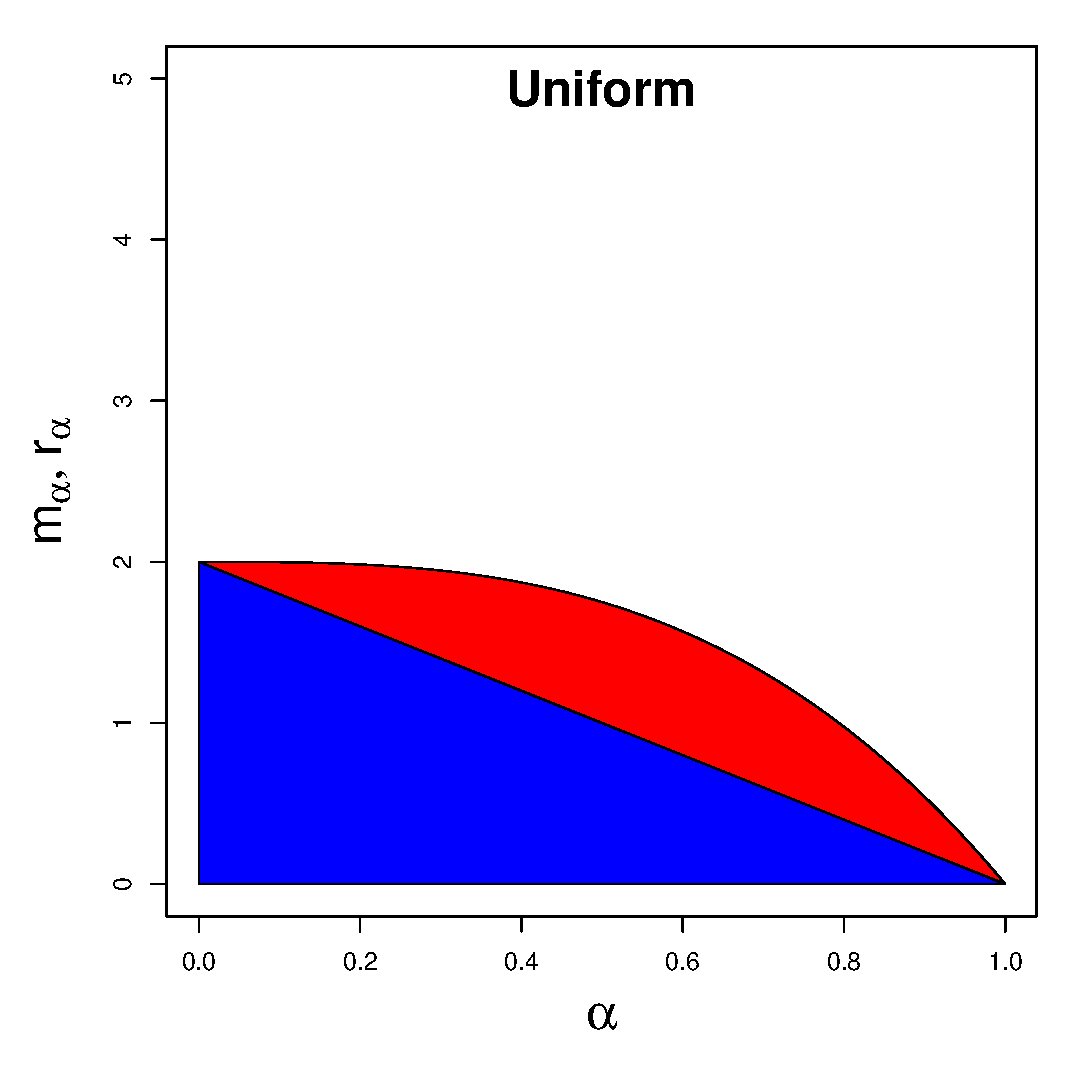
\includegraphics{unirisk.eps}}
      \resizebox{60mm}{!}{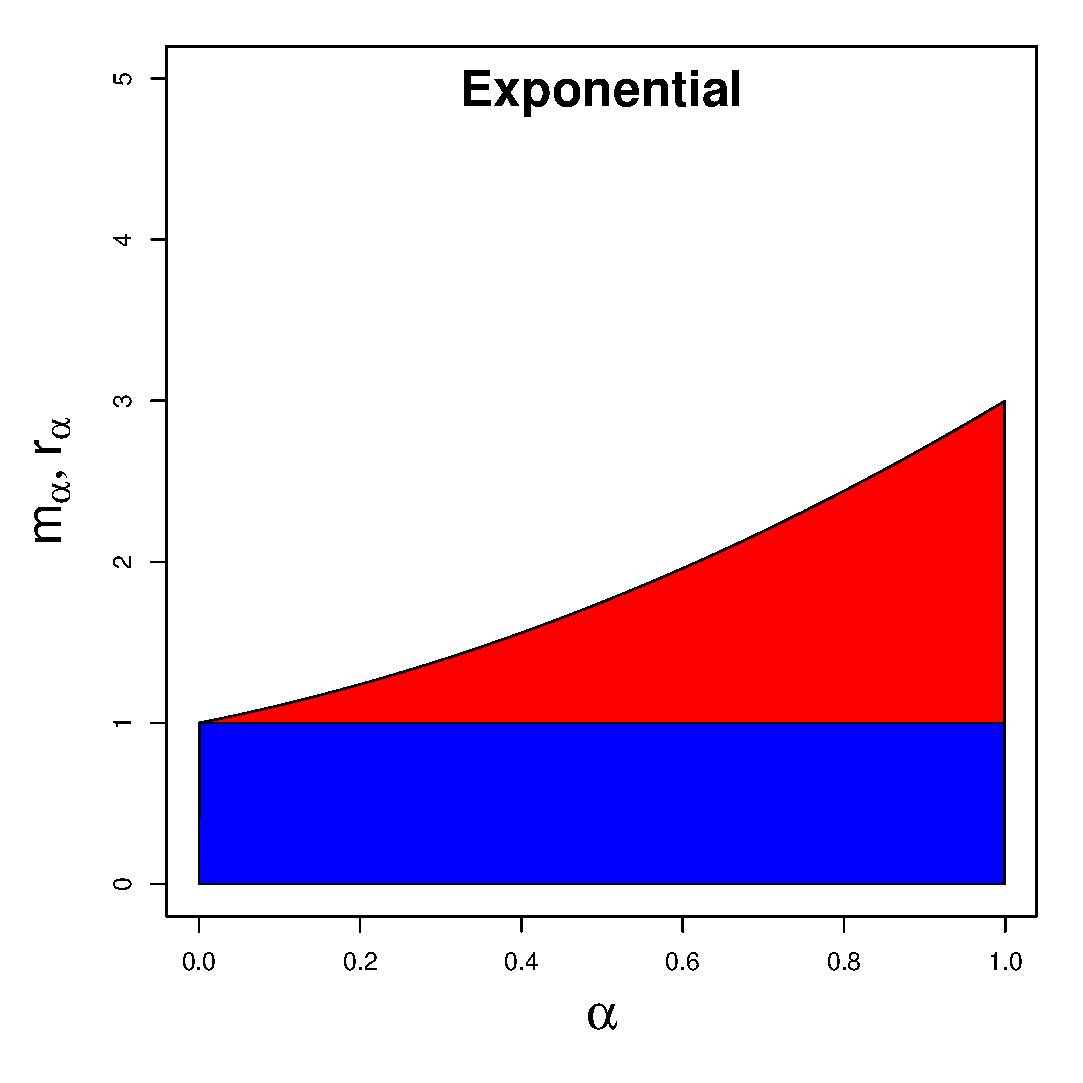
\includegraphics{exprisk.eps}} \\
      \resizebox{60mm}{!}{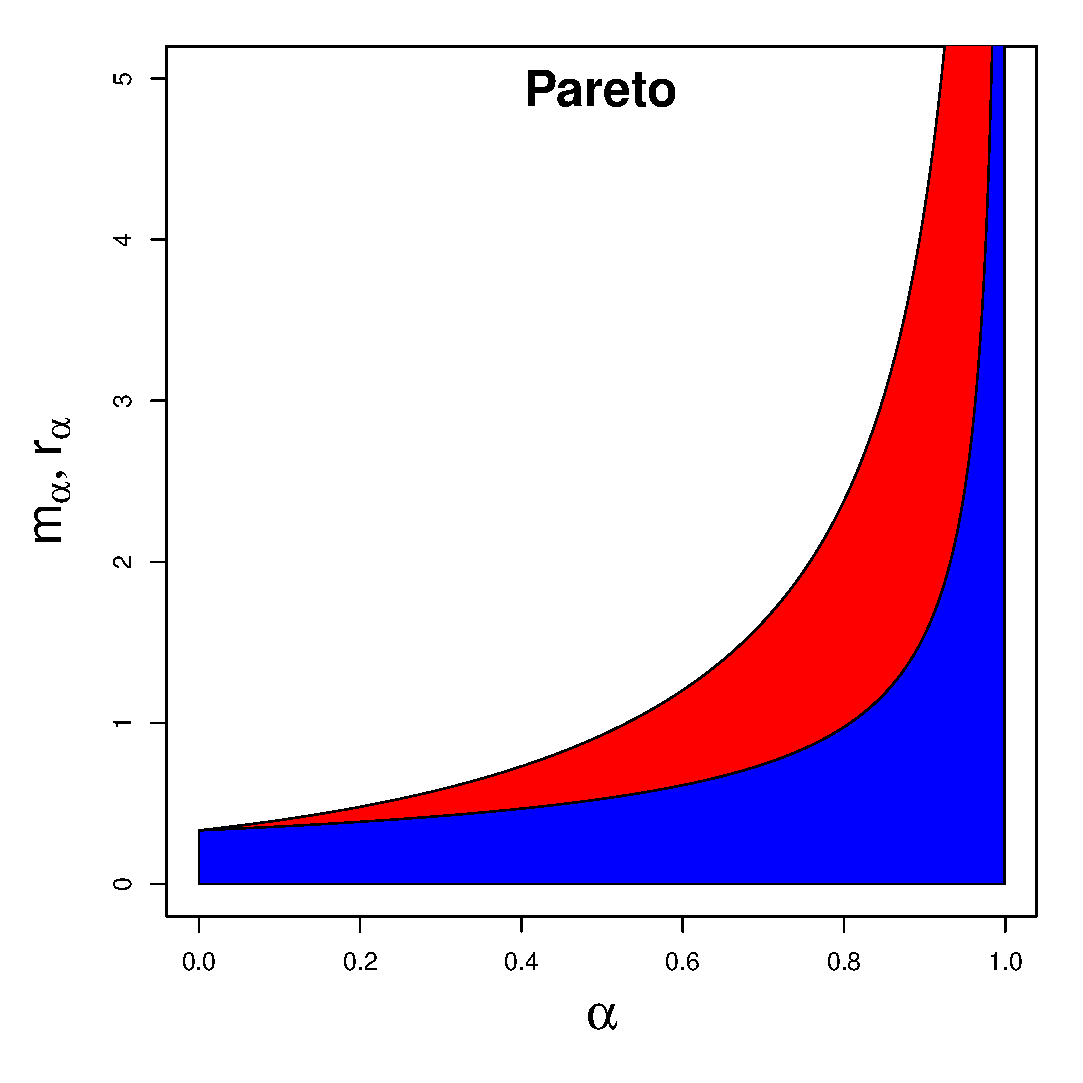
\includegraphics{parrisk.eps}}
      \resizebox{60mm}{!}{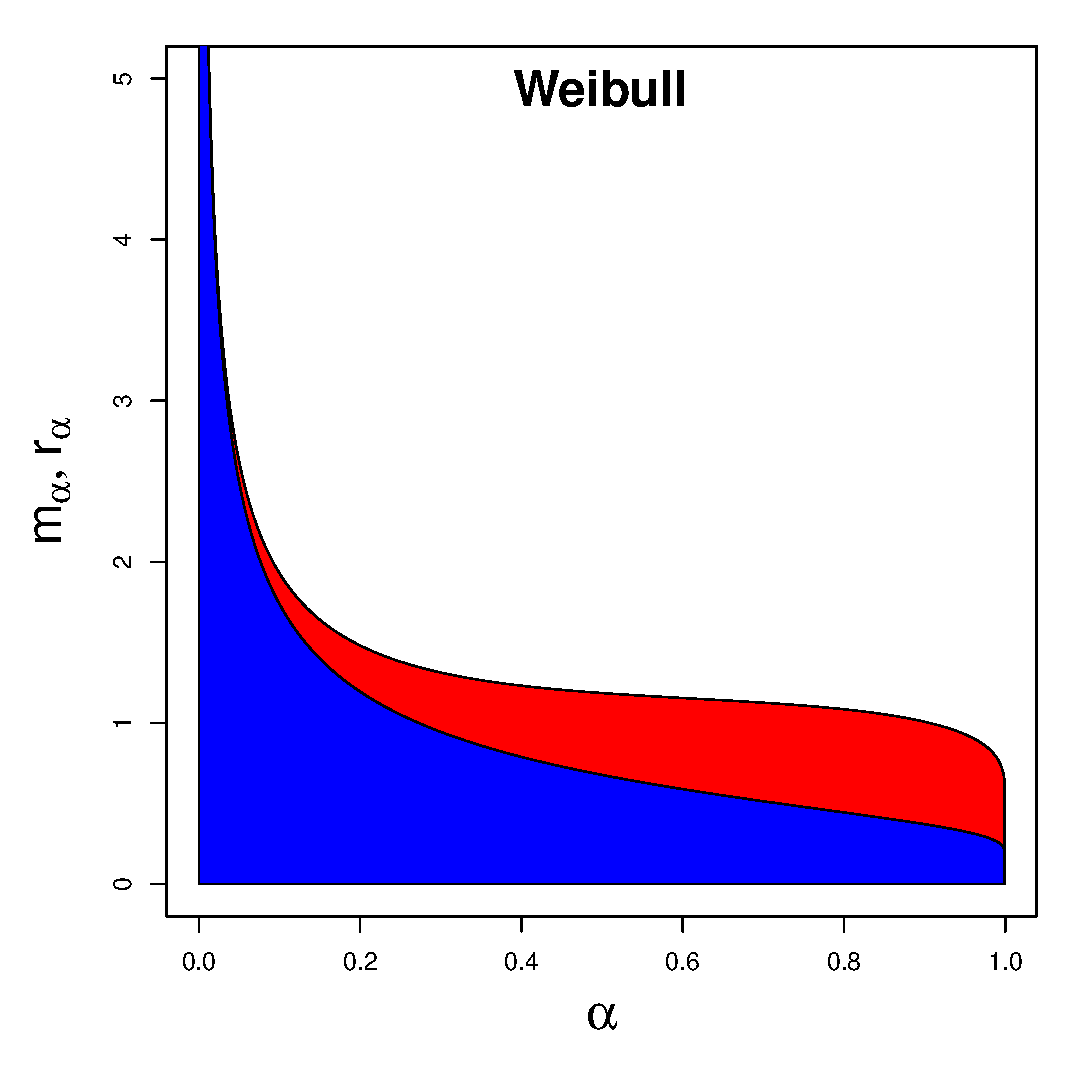
\includegraphics{weirisk.eps}} \\
    \end{tabular}
    \caption{Mean densities (blue area) and risk densities (red area) for the $4$ loss distributions in \fref{fmeancont}. The distortion operator is $\Phi(\alpha)=\alpha^3$ and the risk ratio is $r_\alpha^*=\alpha(1+\alpha)$. }
    \label{frisk}
  \end{center}
\end{figure}


\section{Properties of risk densities and risk ratios}\label{sproprisk}


\subsection{Unique characterisation of distortion operator}


Risk ratios $r_\alpha^*$ over $0\le\alpha\le 1$ uniquely characterise the distortion operator $\Phi$. Given $r_\alpha^*$, re-arranging \eref{riskratio} yields the distortion operator
$$
\Phi(\alpha)=\alpha-(1-\alpha)r_\alpha^* \;.
$$
Thus an alternative formulation of $\Phi$ is to first specify risk ratios across all VaR--layers and then set $\Phi$ using the above result. The condition $\Phi(0)=0$ requires $r_0^*=0$ and $\Phi(1)=1$ is satisfied generally. Increasing and convex $\Phi$ respectively require $1+r_\alpha^*-(1-\alpha)(r_\alpha^*)'\ge0$ and $2(r_\alpha^*)'-(1-\alpha)(r_\alpha^*)''\ge0$.


\subsection{Monotonic loss transformations}

Similar to mean densities, straightforward changes apply to risk densities under monotonic loss transformations. Again assume $y=g(x)$ is an increasing transformation. The risk density of $y$ is
$$
r_\alpha(y)=m_\alpha(y) r_\alpha^* = m_\alpha(x) g'\{V_\alpha\} r_\alpha^* = r_\alpha(x) g'\{V_\alpha(x)\}
$$
where $r_\alpha(x)$ is the risk density of $x$ and noting risk ratios $r_\alpha^*$ are independent of the loss distribution and hence unchanged. Therefore mean and risk densities change identically under increasing transforms. In addition risk densities are proportional to the scale of the loss distribution, similar to mean densities.

Similarly if $g$ is decreasing then the risk density of $y$ is $r_{1-\alpha}(x)g'\{V_{1-\alpha}(x)\}$.



\begin{comment}

\section{Volatility density and volatility ratio}\label{svolatility}


Volatility densities are similar to risk densities and indicate the volatility of each VaR layer. Volatility is measured by standard deviation. Unlike risk densities, volatility densities do not integrate to the overall loss standard deviation. This paper focuses on risk densities due to their additivity. In addition distortion risk captures the skewness of loss distributions, and standard deviation is a more appropriate risk measure for symmetric distributions.

The volatility density is the standard deviation of $\ell_\alpha$:
\begin{equation}\label{volatility}
s_\alpha \equiv \sqrt{\var(\ell_\alpha)} = \sqrt{\alpha(1-\alpha)}V_\alpha' \;,
\end{equation}
since the $\mathrm{VaR}_\alpha$ layer is Bernoulli distributed with probability $1-\alpha$ and scale $V_\alpha'$. The volatility ratio is the ratio between volatility and mean densities:
$$
s_\alpha^* \equiv \frac{s_\alpha}{m_\alpha} = \frac{\sqrt{\alpha(1-\alpha)}V_\alpha'}{(1-\alpha)V_\alpha'} = \sqrt{\frac{\alpha}{1-\alpha}} \;,
$$
and is the coefficient of variation of $\ell_\alpha$. Similar to risk ratios, volatility ratios are increasing and are independent of the loss distribution. Volatility ratio starts at zero at the bottom VaR layer, and increases to infinity at the top VaR layer.

Integrating $s_\alpha$ over $[a,b]$ yields the volatility of the $[a,b]$-VaR layer:
$$
S_{[a,b]} \equiv \int_a^b \sqrt{\alpha(1-\alpha)}V_\alpha' \de \alpha
= \sqrt{b(1-b)}V_b-\sqrt{a(1-a)}V_a
$$
$$
- \int_a^b \frac{0.5-\alpha}{\sqrt{\alpha(1-\alpha)}} V_\alpha \de\alpha \;.
$$
The first integral above is a weighted sum of VaR spacings between $a$-VaR and $b$-VaR, where weights are symmetric about, and highest at, the median. Larger $S_{[a,b]}$ implies greater volatility over the $[a,b]$-VaR layer. In addition $S_{[a,b]}$ is an upper bound on the standard deviation of the $[a,b]$-VaR layer:
\begin{equation}\label{bound}
\sqrt{\var\left( L_{[a,b]}\right)} \le S_{[a,b]}  \;,
\end{equation}
since the standard deviation of a sum ($L_{[a,b]}$) is less than the sum of standard deviations ($S_\alpha$). VaR layers are comonotonic but not linearly dependent, hence equality in \eref{bound} does not hold in general.

When $a=0$ and $b=1$ the integral of the volatility density is
$$
S_{[0,1]} = \int_0^1 \frac{\alpha-0.5}{\sqrt{\alpha(1-\alpha)}} V_\alpha \de\alpha  = \int_{0.5}^1 \frac{\alpha-0.5}{\sqrt{\alpha(1-\alpha)}} \left(V_\alpha-V_{1-\alpha} \right) \de \alpha \ge \sqrt{\var(x)} \;.
$$
Hence overall loss volatility as measured by the volatility density is the weighted difference between VaRs above and below the median, and in general exceeds the loss standard deviation.

\end{comment}






\section{Empirical calculations of mean and risk densities}\label{sempirical}

It is common for insurance and financial companies to collect data or simulate future outcomes to make risk management decisions. Given an ordered sample of losses $\ell_1,\ldots,\ell_n$, calculate mean and risk densities as follows:
\bi
\i Set empirical VaRs equal to ordered observations: $\hat{V}_{i/n}=\ell_i$. The $V_{i/n}$--layer is $I_{\ell_i}(x)(\ell_{i+1}-\ell_i)$ where $x$ is a random observation.

\i The empirical mean density is $\hat{m}_{i/n}=(1-i/n)\hat{V}_{i/n}'$, for $i=0,\ldots,n-1$ where the empirical derivative $\hat{V}_{i/n}'=n(\hat{V}_{(i+1)/n}-\hat{V}_{i/n})$ and $\hat{V}_0=0$.

\i Risk ratios are computed using the specified distortion operator: $r_{i/n}^*=\{i/n-\Phi(i/n)\}/(1-i/n)$. The empirical risk density is $\hat{r}_{i/n}=\hat{m}_{i/n}*r_{i/n}^*$.

\i If necessary, apply parametric or non-parametric smoothing to empirical mean and risk densities to reveal underlying patterns.
\ei
As $n\rightarrow \infty$, empirical VaRs approach true VaRs and the above algorithm converges: $\hat{m}_{i/n}\rightarrow m_\alpha$ and $\hat{r}_{i/n}\rightarrow r_\alpha$ where $\alpha=i/n$.

Overall mean and risk are the respective sums (rather than integrals)
$$
\sum_{i=0}^{n-1} \frac{m_{i/n}}{n} \cq \sum_{i=0}^{n-1} \frac{r_{i/n}}{n}
\;.
$$
Taking sums over other subsets yield mean and risk over corresponding VaR--layers. In addition manipulating the first summation above yields the arithmetic mean $\sum_{i=1}^n \ell_i /n$ of the loss sample.

The following calculates mean and risk densities from NASDAQ, S\&P and FTSE daily returns between 1985 and 2015 assuming a stationary distribution. Form a hypothetical portfolio of \$100 in each market index. Focus on daily investment losses rather than gains, hence switch the signs of historical returns and gains are treated as negative losses. In addition apply the distortion operator $\Phi(\alpha)=I_c(\alpha)(\alpha-c)/(1-c)$ where $c=0.75$, implying overall risk is the difference between expected losses above VaR$_{0.75}$ and the overall mean. Note the condition $x\geq 0$ is relaxed in this illustration, as the interest is in the shape of mean and risk densities rather than their actual values.

\fref{fcase} illustrates results. Empirical densities and VaRs of daily investment losses are shown in addition to empirical mean and risk densities. The following are key observations:
\bi

\i NASDAQ has more skewed losses and gains than S\&P and FTSE, and in particular larger VaR--spacings. As a result NASDAQ has larger mean and risk densities, and larger mean loss and risk overall. S\&P and FTSE behave similarly particularly in the tails.

\i Empirical mean densities are large at low VaR--layers, then decrease rapidly at higher VaR--layers. High mean density values at low layers are formed by large VaR--spacings in left tails of loss distributions. 

\i Relatively stable mean densities at higher VaR--layers indicate upper tails of loss distributions have similar shape as the exponential distribution.

\i Empirical risk densities paint a different picture from mean densities: risk is mainly contributed by higher layers, unlike for the mean. This observation is consistent with common knowledge that extreme market losses, whilst rare, contribute significantly to portfolio volatility.
\ei
\begin{figure}
  \begin{center}
    \begin{tabular}{cc}
      \resizebox{60mm}{!}{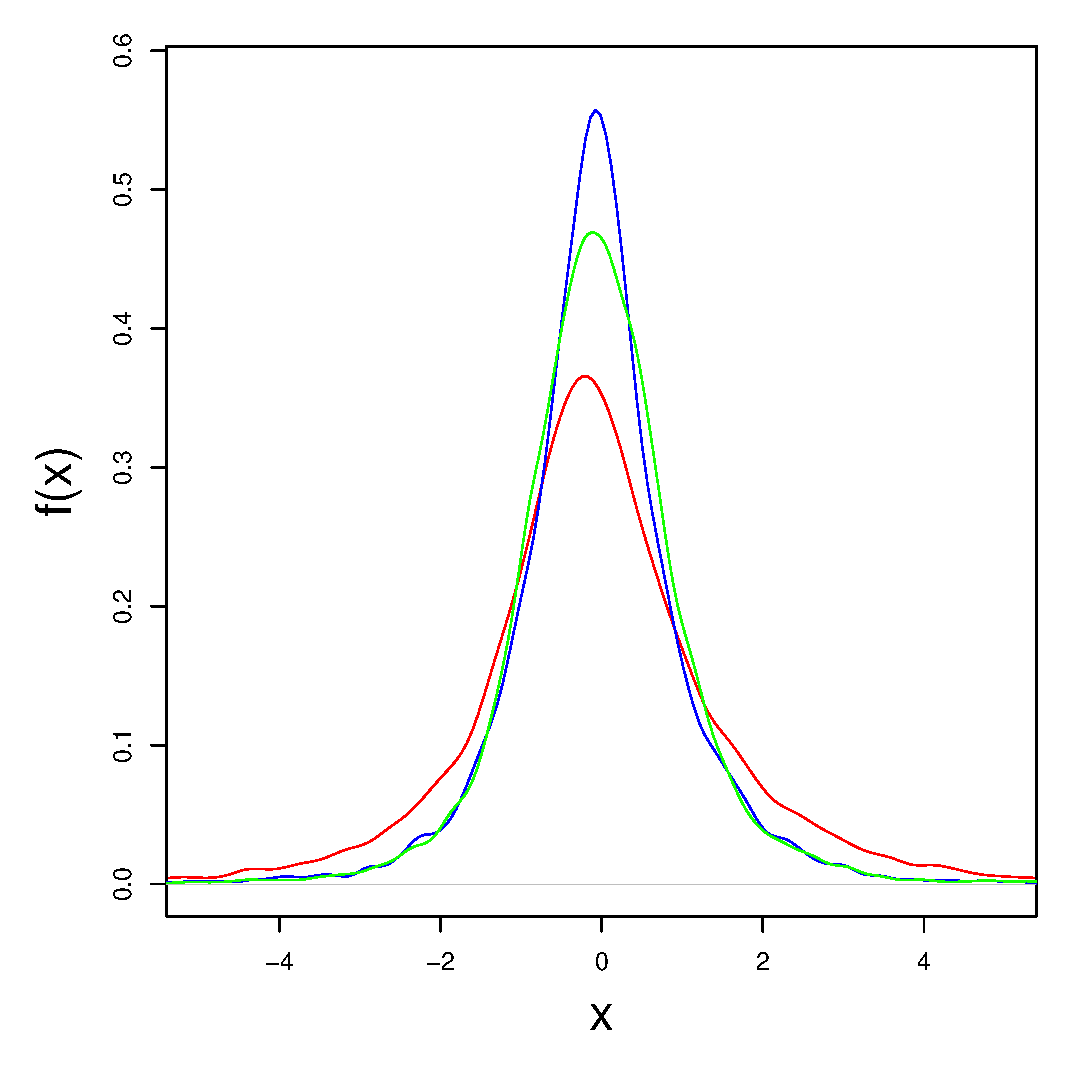
\includegraphics{density.eps}}
            \resizebox{60mm}{!}{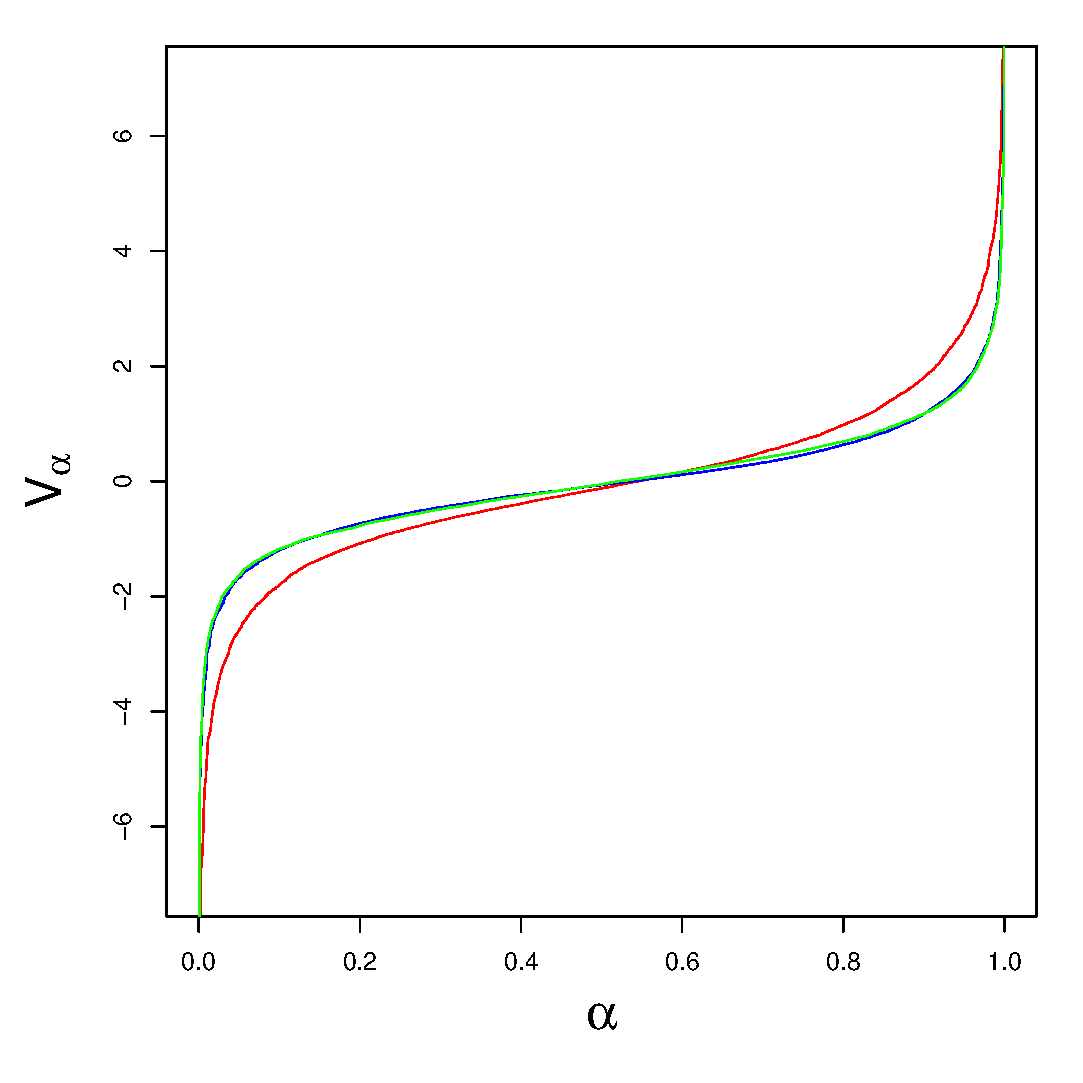
\includegraphics{quantile.eps}}\\
       \resizebox{60mm}{!}{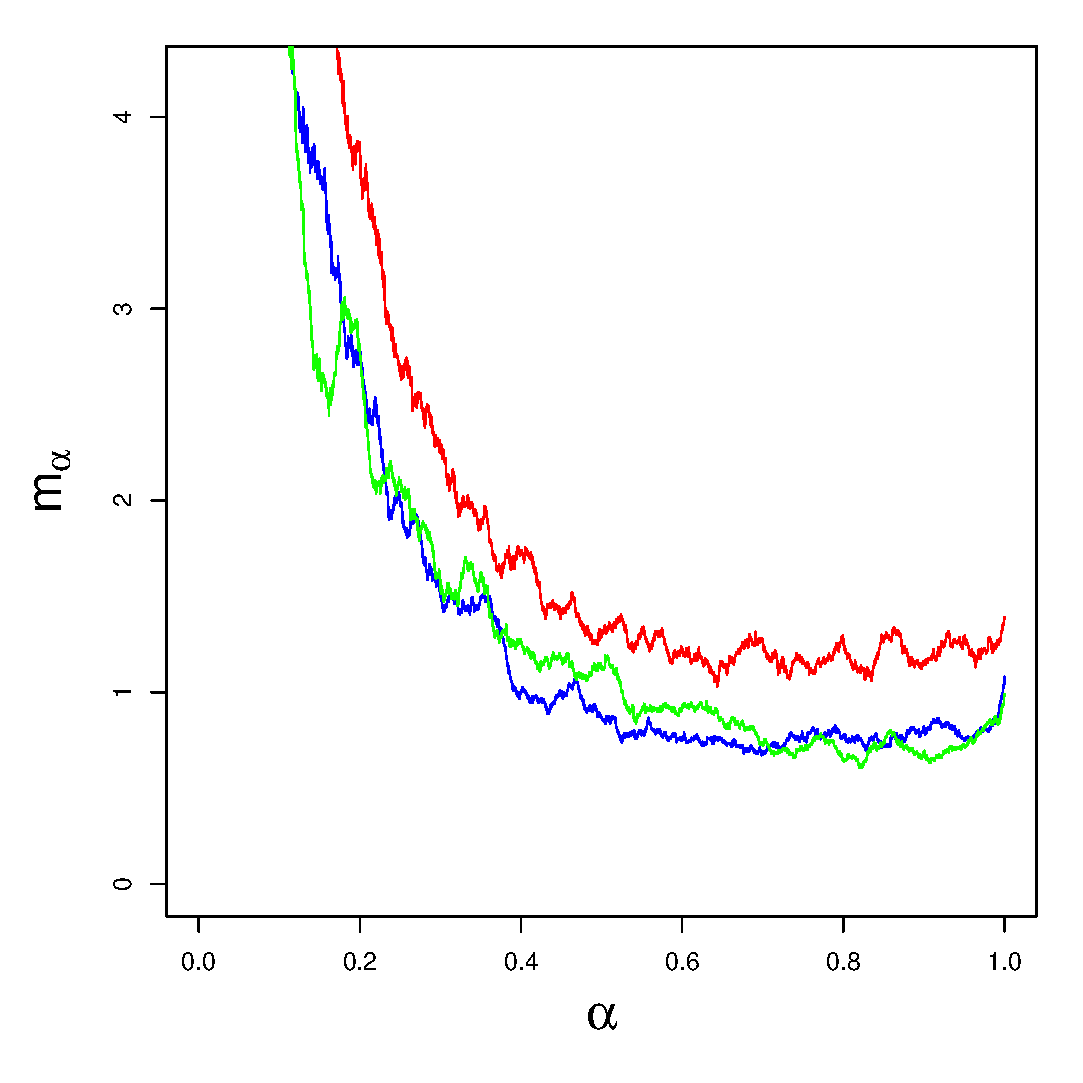
\includegraphics{mean.eps}}
              \resizebox{60mm}{!}{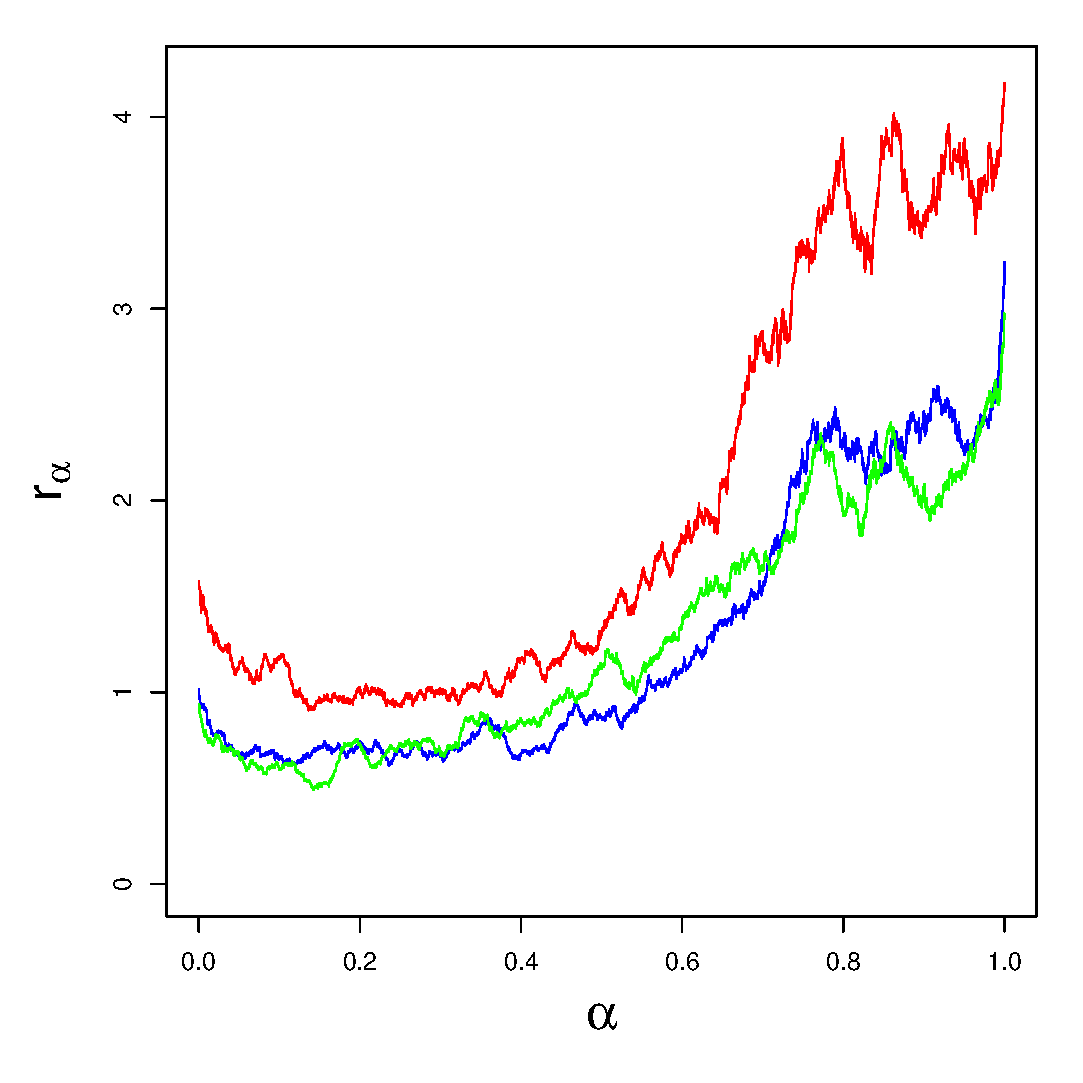
\includegraphics{risk.eps}}\\
    \end{tabular}
    \caption{Top left and right panels plot empirical loss densities and distributions, respectively. Bottom left and right panels plot smoothed empirical mean and risk densities, respectively. Red, blue and green represent NASDAQ, S\&P and FTSE, respectively.}
    \label{fcase}
  \end{center}
\end{figure}


\section{Applications of mean and risk densities}\label{sapplication}


Remaining sections apply mean and risk densities to common risk management problems involving reinsurance, capital buffers and debt tranching. Current statistical tools provide identical solutions in some cases. However mean and risk densities offer a more elegant solution and yield additional insights.

\begin{comment}
Capital covers adverse loss outcomes. Capital is usually set equal to VaR with a fixed threshold. For example Solvency II insurance regulation references $90\%$ and $99.5\%$ VaRs \citep{eling2007solvency}. VaR based capital limits the probability of shortfall -- $10\%$ and $0.5\%$ respectively in Solvency II. VaR based capital adjusts to the shape and scale of the loss distribution. Given a fixed threshold, VaR increases with scale and skewness of the loss distribution.
\end{comment}



\section{Pricing and insuring loss layers}

Suppose the $[V_\alpha,V_\beta]$ VaR--layer of loss $x$ is insured or reinsured. Hence $V_a$ is the excess and $V_b$ is the limit of the coverage. The premium is
$$
P = \int_\alpha^\beta (m_\pi+ r_\pi) \de \pi =  \int_\alpha^\beta \{1-\pi+\pi-\Phi(\pi) \} V_\pi' \de \pi
=\int_\alpha^\beta \{1-\Phi(\pi) \} V_\pi' \de \pi
$$
$$
= \{1-\Phi(\beta)\}V_\beta-\{1-\Phi(\alpha)\}V_\alpha + \int_\alpha^\beta V_\pi \Phi'(\pi) \de \pi  \;,
$$
where $\int_\alpha^\beta m_\pi\de \pi$ is the pure premium and $\int_\alpha^\beta r_\pi\de \pi$ is the risk loading forming the overall premium $P$. Both components increase as coverage widens: lower $\alpha$ or higher $\beta$. Changes to overall premium due to changes in the excess or limit are the partial derivatives
$$
\frac{\partial P}{\partial \alpha}  = -(m_\alpha+ r_\alpha)
\cq \frac{\partial P}{\partial \beta}  = m_\beta+ r_\beta
\;.
$$
The previous illustration in \fref{frisk} shows the pure premium and risk loading for various $\alpha$ and $\beta$ assuming uniform, exponential, Pareto and Weibull loss distributions and the distortion operator $\Phi(\alpha)=I_c(\alpha)(\alpha-c)/(1-c)$. The overall premium is the total area over $[\alpha,\beta]$. For example, for an exponential loss distribution, the pure premium increases at the same rate as the excess and limit are changed. However the risk loading increases at an increasing rate when the limit increases, and forms a larger component of the overall premium when high VaR--layers are insured.

Intuitively, the purchaser of insurance or reinsurance would select an excess and limit covering the bulk of the area under mean and risk densities. This implies higher excesses and limits for exponential and Pareto loss distributions. On the other hand, lower excesses and limits would suffice for uniform (and potentially Weibull) loss distributions, as higher layers have lesser mean and risk contributions. The optimal excess and limit depends on the interaction between the premium cost, the purchaser's budget and utility function.



\begin{comment}
\section{Setting limits on insured loss}

Insurers typically impose a limit $V_l$ on an insured loss to manage risk. The following proposes a solution for $l$. Suppose a profit margin $\pi$ is charged on the mean loss $M_{[0,l]}$, noting only the $[0,l]$-VaR layer is insured. The insurer's risk is $R_{[0,l]}$ with cost $k R_{[0,l]}$, where $k$ is the cost per unit risk. If $R_{[0,l]}$ is the capital held then $k$ is the cost of capital.

A profitable $l$ ensures profit margin exceeds cost of risk in dollar terms:
$$
\pi M_{[0,l]} \geq k R_{[0,l]} \cq \frac{R_{[0,l]}}{M_{[0,l]}} = R_{[0,l]}^* \leq \pi/k
$$
where $R_{[0,l]}^*$ is the risk ratio over the $[0,l]$-VaR layer. Since $R_{[0,l]}^*$ increases in $l$, $l$ is set to ensure that the insurer's risk ratio does not exceed $\pi/k$, the ratio between profit margin and cost per unit risk. Higher $\pi$ or lower $k$ permits higher loss limit. Write the risk ratio $R_{[0,l]}^*$ as
$$
R_{[0,l]}^* = \frac{\int_0^l m_\alpha r^*_\alpha \de \alpha }{\int_0^l m_\alpha \de\alpha} \cq r^*_\alpha=\frac{\alpha-\Phi(\alpha)}{1-\alpha}
$$
where $r_\alpha^*$ increases with $\alpha$ and is independent of the loss distribution. A skewed loss distribution with increasing mean density emphasizes larger values of $r_\alpha^*$, and thus has higher $R_{[0,l]}^*$ given $l$. This implies skewed loss distributions require a lower loss limit.

If $l$ is arbitrarily set then positive profitability requires profit margin
$$
\pi \geq k \frac{R_{[0,l]}}{M_{[0,l]}} \;,
$$
the product of the risk cost and risk ratio over $[0,l]$-VaR layer. Increasing either component increases the profit margin.
\end{comment}


\section{Credit quality of debt tranches}

Consider a debt with fixed principal $p$ and random default loss $0\le x\le p$. The credit rating of the debt is typically based on the following quantities:
$$
\textrm{PD}=\p(x>0) \cq \textrm{PEL}=\frac{\E(x)}{p} \cq \textrm{RR}=\frac{r}{\E(x)}
$$
where PD is the default probability, PEL is the expected default loss as a proportion of principal and RR is the risk of the default loss relative to its mean value. A high credit rating may be issued for example if a combination of PD, PEL and RR falls below specified limits \citep{das2011differences}.


Suppose the debt is split into tranches. The default loss on the tranche from $V_\alpha$ to $V_\beta$ is $\max\{\min(x-V_\alpha,0),V_\beta-V_\alpha\}$ and is hence the VaR--layer $[V_\alpha,V_\beta]$ of $x$. The principal of this tranche is layer width $V_\beta-V_\alpha$. In addition $V_\alpha$ and $V_\beta$ are called the attachment and detachment points of the tranche, respectively. There is a default loss if $x>V_\alpha$, and a complete loss of principal if $x\ge V_\beta$.


Splitting a debt into tranches is used in securitisation to enhance the credit quality of portions of the debt \citep{mandel2012role}. Debt tranches are common in collaterised debt obligations \citep{duffie2001risk}. Lower, junior tranches are more likely to suffer a default loss and are assigned a lower credit rating. Higher, senior tranches only suffer default losses after losses have passed through junior tranches and hence typically receive a higher credit rating.


Corresponding credit rating statistics for the tranche or layer $[V_\alpha,V_\beta]$, using mean and risk densities defined in \eref{meancont} and \eref{riskcont}, are
$$
\textrm{PD}=\p(x>V_\alpha)=1-\alpha \cq
\textrm{PEL}=\frac{\int_\alpha^\beta m_\pi \de \pi}{V_\beta-V_\alpha} = \frac{\int_\alpha^\beta (1-\pi)V_\pi' \de \pi}{\int_\alpha^\beta V_\pi' \de \pi}  \;,
$$
$$
\textrm{RR} = \frac{\int_\alpha^\beta r_\pi \de \pi}{\int_\alpha^\beta m_\pi \de \pi}
=\frac{\int_\alpha^\beta r_\pi^* m_\pi \de \pi}{\int_\alpha^\beta m_\pi \de \pi}  \;,
$$
where as before $V_\pi'$ is the derivative of $V_\pi$ with respect to $\pi$ and $r_\pi^*=r_\pi/m_\pi$ is the risk ratio of the $V_\pi$--layer of $x$. Hence PEL is a weighted average of default probabilities $1-\pi$ from $\pi=\alpha$ to $\beta$, where weights are VaR derivatives or spacings. Setting $\beta \rightarrow\alpha$ leads to PEL$\rightarrow 1-\alpha$ which is the PD. RR is a weighted average of risk ratios from $\alpha$ to $\beta$. Note PEL in this case is also the rate-on-line in excess-of-loss reinsurance ignoring the risk loading.

Both PD and PEL on tranche $[V_\alpha,V_\beta]$ decrease as $\alpha$ or $\beta$ increases. Hence the probability and expected proportion of default are smaller for higher tranches, consistent with common knowledge. However RR increases since $r_\pi^*$ is increasing in $\pi$. Hence the default loss becomes riskier in higher tranches, even though a default loss is less likely and on average smaller. In addition, as default losses on tranches are comonotonic, there is no diversification benefit from holding multiple tranches originating from the same loss. This lack of diversification is a reason for catastrophic financial losses during the 2008 crisis \citep{kolb2010lessons}. 



\section{Setting capital buffers}


Suppose capital $V_c$ is held to cover loss $x$. There is a shortfall if $x>V_c$ and surplus if $x\le V_c$. The capital shortfall is the VaR--layer $[V_c,V_1]$ of $x$ and capital consumed is the VaR--layer $[0,V_c]$. The following derives $c$ or $V_c$ in two different ways, using mean and risk densities.


\subsection{Limiting expected shortfall}


Suppose capital $V_c$ is held to restrict expected shortfall to a proportion $s$ of overall expected loss where $s$ is small, say 1\%. Hence $c$ is solved from
\begin{equation}\label{shortfall}
\frac{\E(L_1-L_c)}{\E(L_1-L_0)} = \frac{\int_c^1 m_\alpha\de\alpha}{\int_0^1 m_\alpha\de\alpha} = s  \;.
\end{equation}
An equivalent standard statistical expression is
$$
\frac{\E\{\max(x-V_c,0)\}}{\E(x)} = s \;.
$$
Equation \eref{shortfall} implies $c$ is selected so that the relative area under the upper tail of mean density $m_\alpha$ is $s$. \fref{fcapital} provides an illustration using a Weibull loss distribution. Smaller $s$ requires higher $c$ and $V_c$.

A similar, common approach is to set capital to restrict the \textit{probability} of shortfall, as opposed to \textit{expected} shortfall, to say again $s$. Under this approach, capital is selected such that the upper tail area under the probability density (rather than the mean density) is $s$. It is straightforward to show that required capital is $V_{1-s}$. This approach is also illustrated in \fref{fcapital}. Insurance and banking regulations typically set capital at $V_{1-s}$ with pre-determined $s$ (\cite{eling2007solvency}, \cite{chernobai2008operational}).


\begin{figure}
  \begin{center}
    \begin{tabular}{cc}
      \resizebox{60mm}{!}{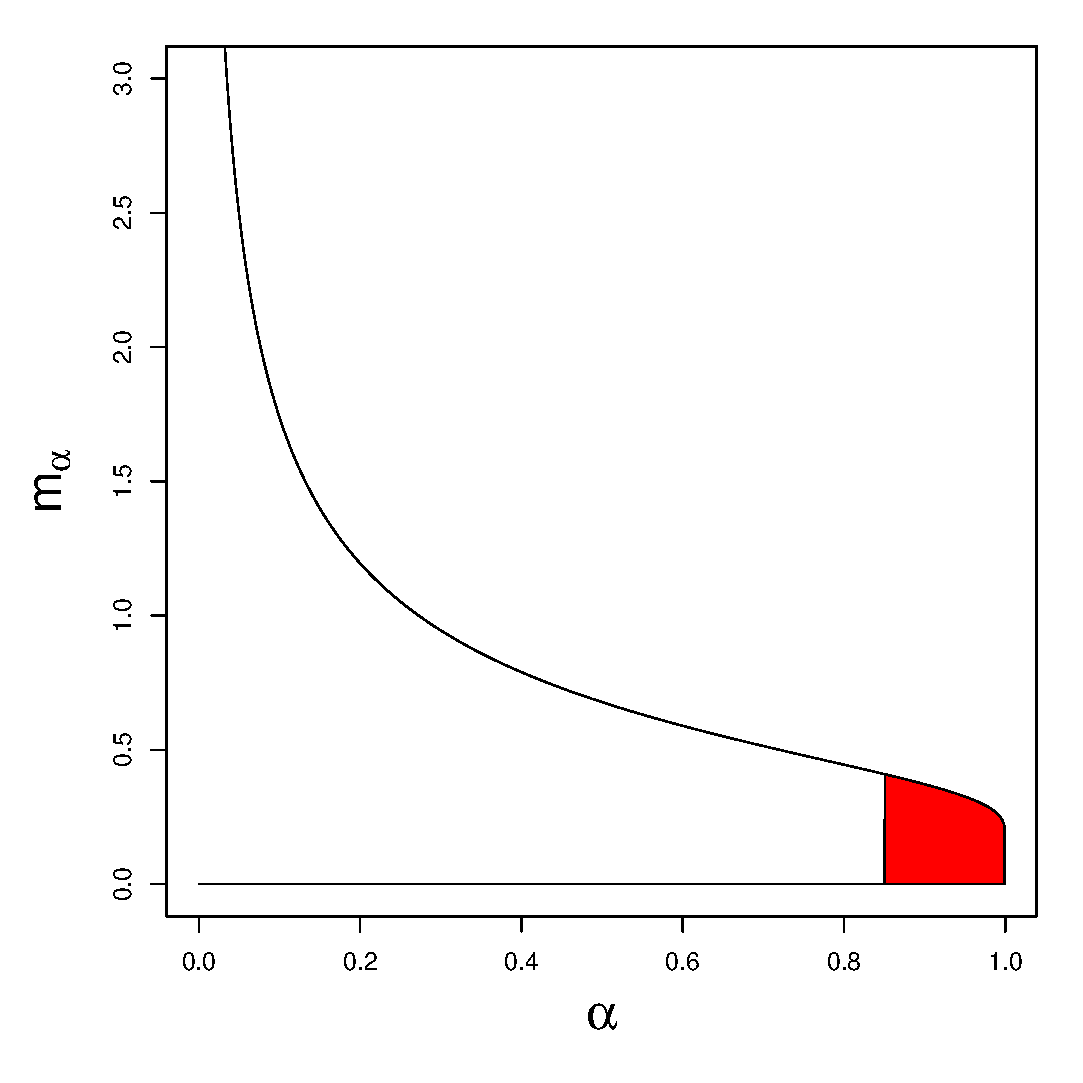
\includegraphics{shortfallcap.eps}}
      \resizebox{60mm}{!}{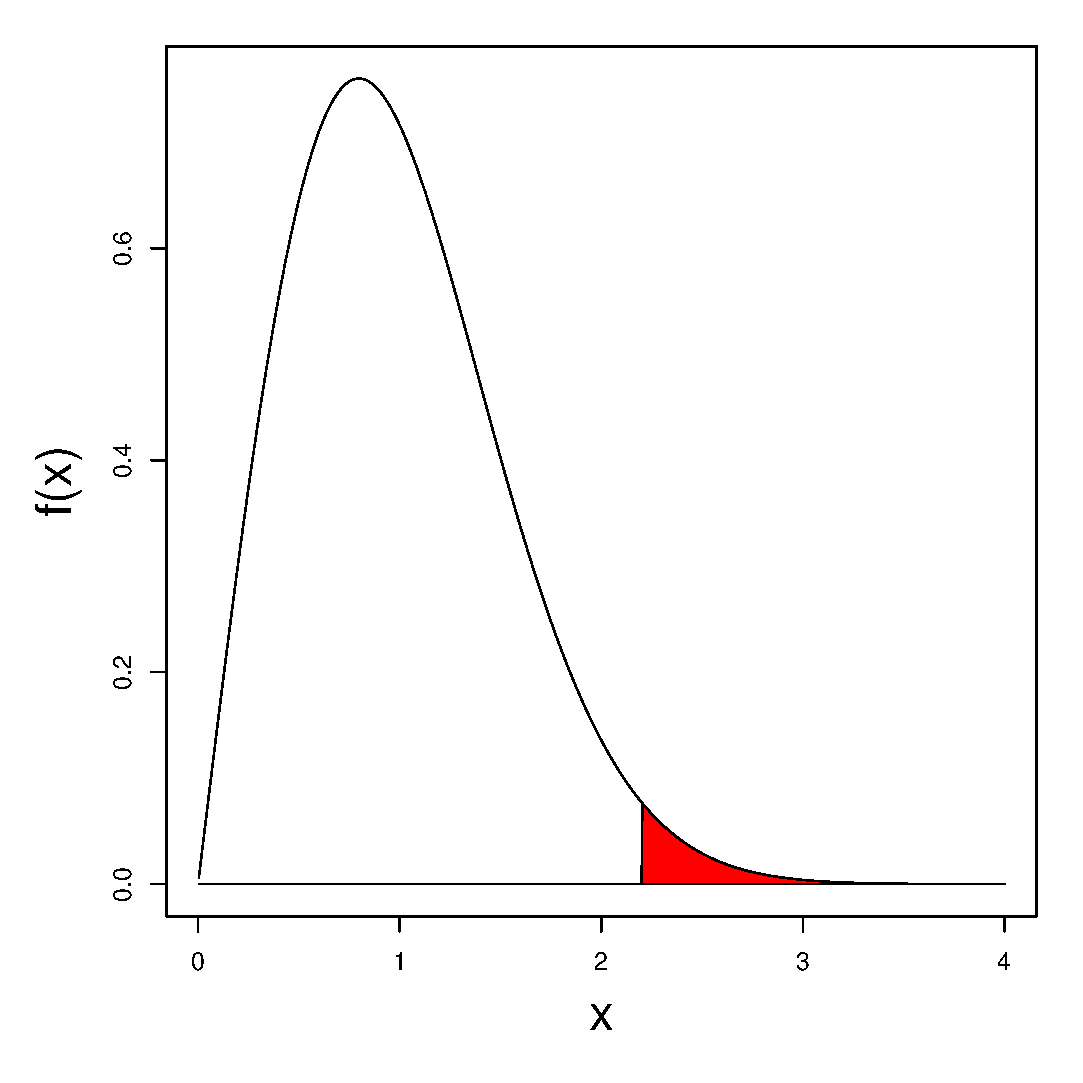
\includegraphics{varcap.eps}} \\
    \end{tabular}
    \caption{The left panel shows capital with fixed expected shortfall as a proportion of overall expected loss (red area under the mean density). The right panel shows capital with fixed shortfall probability (red area under the probability density).}
    \label{fcapital}
  \end{center}
\end{figure}

Setting capital based on expected shortfall is more appropriate than using shortfall probability as the shape of the loss distribution is reflected. This is demonstrated by the following examples. For an exponential loss distribution, the mean density is flat (see \sref{smeaneg}) and \eref{shortfall} reads $1-c=s$ therefore capital is $V_{1-s}$. For example if expected shortfall is 1\% of overall mean loss then capital is $V_{0.99}$. Setting shortfall probability at $s$ also yields capital $V_{1-s}$, hence both approaches are the same for exponential loss distributions. For a Pareto loss distribution with shape parameter $\gamma$, solving \eref{shortfall} yields
$$
\int_c^1 \frac{1}{(1-\alpha)^{1/\gamma}} \de \alpha =
s \int_0^1 \frac{1}{(1-\alpha)^{1/\gamma}} \de \alpha \cq
c=1-s^{\gamma/(\gamma-1)} \ge 1-s \;.
$$
In this case capital $V_c\ge V_{1-s}$. Therefore referring to expected shortfall rather than shortfall probability increases capital. The reason is the Pareto distribution has a thicker upper tail than the exponential, hence increasing expected shortfall. Reducing the skewness of the Pareto by increasing $\gamma$ reduces $V_c$. Generally for an increasing mean density, $\int_{1-s}^1 m_\alpha\de\alpha > s \int_0^1 m_\alpha\de\alpha$ thus $c>1-s$, and vice versa for a decreasing mean density. Hence when capital is set based on expected shortfall, the capital VaR threshold varies with the shape of the loss distribution. Higher skewness requires a higher VaR threshold and reduces shortfall probability. On the other hand a higher shortfall probability is appropriate for a less skewed loss distribution.

Extend \eref{shortfall} by replacing expectations with risk-adjusted expectations. Then $c$ is solved from
\begin{equation}\label{shortfall1}
\frac{\Ex(L_1-L_c)}{\Ex(L_1-L_0)}
= \frac{\int_c^1 (m_\alpha+r_\alpha)\de \alpha}{\int_0^1 (m_\alpha+r_\alpha)\de \alpha}
= \frac{\int_c^1 m_\alpha(1+r^*_\alpha)\de \alpha}{\int_0^1 m_\alpha(1+r^*_\alpha)\de \alpha}
= s \;.
\end{equation}
Since $r_\alpha^*$ is increasing in $\alpha$, $m_\alpha(1+r_\alpha^*)$ increases at a relatively faster rate than $m_\alpha$. For example refer to the exponential loss distribution in \fref{fmeancont}. The mean density is flat but increasing after risk adjustment. Hence $c$ from \eref{shortfall1} exceeds $c$ from \eref{shortfall}, using the above argument. Risk-adjusted expected shortfall increases relative to overall risk-adjusted expected loss, resulting in higher $c$.


The scale of the loss distribution does not affect $c$ in \eref{shortfall} and \eref{shortfall1}, since scale factors are present in numerator and denominator. Scale is reflected when $V_c$ is computed from $c$. Also note that a consequence of expressing loss layers as VaR layers is that derived quantities are in VaR terms rather than in dollars. This argues for VaR layers given the prevalence of VaR references in practice.



\subsection{Balancing expected shortfall and surplus}


The following derives capital by considering expected capital surplus in addition to shortfall. Considering capital surplus recognises opportunity costs of holding capital. All else equal, a higher opportunity cost reduces capital held.


Suppose an opportunity cost $i$ is attached to every dollar of capital surplus. For example $i$ may be the expected return on alternative investments. Per dollar cost of capital shortfall is $j$, for example the borrowing cost when in distress. Given capital $V_c$, the expected total cost of capital shortfall and surplus expressed in VaR--layers and the mean density is
$$
\Gamma = i \E\left(V_c-L_c\right) + j \E(L_1-L_c) = i \left(V_c-\int_0^c m_\alpha \de \alpha \right) +j \int_c^1 m_\alpha \de \alpha
$$
$$
=i\E\{\max(V_c-x,0)\} + j\E\{\max(x-V_c,0)\} \;,
$$
where the final expression uses standard statistical notation and is shown for comparison. Setting the derivative of $\Gamma$ with respect to $c$ to 0 yields
$$
i(V_c'-m_c)-jm_c=0 \cq ic- j(1-c)=0 \cq c=\frac{j}{i+j}  \;.
$$
The middle expression is derived from the first by dividing by $V_c$. Substituting $c=i/(i+j)$ into the second derivative of $\Gamma$ confirms a minimum.

Therefore the capital VaR threshold in this setup is the unit shortfall cost $j$ relative to the total unit cost $i+j$. If $i=j$ then $c=0.5$ and capital is held at the median. Higher $j$ relative to $i$ increases $c$ and $V_c$. In addition any capital $V_c$ implies relative shortfall cost $j/i=c/(1-c)$. For example, capital $V_{0.99}$ implies $j/i=99$, thus the unit cost of shortfall is implicitly $99$ times the unit cost of surplus. Higher $c$ implies higher $j$ relative to $i$.

Again introducing risk-adjustment yields a revised expected total cost
$$
\Gamma = i \left\{V_c-\int_0^c (m_\alpha+r_\alpha) \de \alpha \right\} +j \int_c^1 (m_\alpha+r_\alpha) \de \alpha \;.
$$
Setting the derivative $V_c'[ i\Phi(c)+  j \{1-\Phi(c)\}]=0$ yields $c$ as the solution to
$$
\Phi(c)= \frac{j}{i+j}  \;.
$$
The solution $c>j/(i+j)$ since $\Phi$ is convex or $\Phi(c)\le c$. Risk adjustment hence increases capital since expected shortfall and its cost are magnified relative to surplus. In addition $c$ increases as distortion increases, and reduces to $j/(i+j)$ when there is no distortion. For example the distortion operator $\Phi(c)=c^n$ where $n\ge 1$ yields $c=\{j/(i+j)\}^{1/n}$ which is increasing in $n$ and approaches $1$ as $n\rightarrow \infty$.


The capital VaR threshold $c$ derived by minimising expected cost of shortfall and surplus is independent of the loss distribution. In contrast the first approach where expected shortfall is set as a proportion of expected loss yields a value of $c$ varying with the shape of the loss distribution. In both cases derived capital is expressed directly in VaR terms instead of dollars.


\section{Loss transformation using reinsurance}

The following illustrates how reinsurance transforms the probability, mean and risk profiles of a random loss.


Suppose an insurer faces loss $x$, and enters into a reinsurance arrangement where a portion $0\le t_\alpha\le 1$ of every $V_\alpha$--layer is reinsured and the remaining portion $1-t_\alpha$ is retained. Hence $V_\alpha$--layer and its mean and risk all reduce by $t_\alpha$. The retained loss is formed by combining retained VaR--layers
\begin{equation}\label{reinsurance}
\tilde{x}\equiv \int_0^1 (1-t_\alpha) \de L_\alpha
= \int_0^1 (1-t_\alpha)I_\alpha(u)V_\alpha' \de \alpha
\end{equation}
and the corresponding mean and risk densities are, respectively,
\begin{equation}\label{reinsurance}
\tilde{m}_\alpha \equiv (1-t_\alpha) m_\alpha \cq
\tilde{r}_\alpha \equiv (1-t_\alpha) r_\alpha \;.
\end{equation}
Risk ratios are unchanged after reinsurance: $\tilde{r}_\alpha/\tilde{m}_\alpha=r_\alpha/m_\alpha$. The loss distribution is altered by reinsurance and is further discussed below.

The set of values of $t_\alpha$ over $0\le \alpha\le 1$ defines the ``reinsurance structure." Typical reinsurance structures are ``quota share": $t_\alpha=t$ and ``excess-of-loss": $t_\alpha=I_d(\alpha)$. Quota share covers a constant proportion $t$ of all layers. Excess-of-loss covers all VaR--layers above $d$. A combination of quota share and excess-of-loss can also be applied.

The VaR$_\alpha$--spacing after reinsurance is $\tilde{V}_\alpha'=(1-t_\alpha)V_\alpha'$. Therefore integrate this expression to construct the VaR$_\alpha$ of the retained loss:
$$
\tilde{V}_\alpha = \int_0^\alpha (1-t_s) V_s' \de s = (1-t_\alpha) V_\alpha +\int_0^\alpha V_s t_s' \de s \;,
$$
where the second expression follows from integration by parts. For quota share, $t_\alpha'=0$ therefore $\tilde{V}_\alpha=(1-t)V_\alpha$. Losses reduce by a portion $t$. For excess-of-loss, $t_\alpha'=(\alpha=d)$, the Dirac delta function, and $\tilde{V}_\alpha=\{1-I_d(\alpha)\}V_\alpha + I_d(\alpha)V_d$. Hence all losses below $V_d$ are retained and losses above $V_d$ are capped at $V_d$, implying the retained loss is the VaR--layer $[0,V_d]$ of $x$.

The following constructs a reinsurance structure to yield a target probability, mean or risk profile of the retained loss. If the target mean density is $\tilde{m}_\alpha$ then from \eref{reinsurance} the reinsurance structure is $t_\alpha=1-\tilde{m}_\alpha/m_\alpha$. Similarly for a target risk density. If the target loss distribution has VaR$_\alpha$ $\tilde{V}_\alpha$ then $t_\alpha=1-\tilde{V}_\alpha'/V_\alpha'$. In all cases the reinsurance structure computes the ratio between target and original quantities.

Consider a Pareto loss distribution with shape parameter $\gamma>1$ and scale parameter $b>0$. A reinsurance structure is required to transform the loss distribution into an exponential with scale $\tilde{b}>0$. The reinsurance structure is
$$
t_\alpha = 1-  \frac{\tilde{b}(1-\alpha)^{-1} }{b\gamma^{-1}(1-\alpha)^{-(1/\gamma+1)}}
= 1-\tilde{b}b^{-1}\gamma (1-\alpha)^{1/\gamma}
$$
Hence reinsurance is $1-\tilde{b}b^{-1}\gamma$ at the zero VaR layer, and increases monotonically to $1$ at the highest VaR layer. This result is intuitive since the Pareto is thicker tailed than the exponential. Hence in order to transform the loss from Pareto to exponential, minimum reinsurance is required for small losses and larger losses are increasingly reinsured. Note $\tilde{b}\le b/\gamma$ since $0\le t_\alpha\le 1$.


\begin{comment}
\section{Optimal excess-of-loss reinsurance}

Suppose excess-of-loss reinsurance with excess $d$ is purchased. The problem is to calculate an optimal $d$ for the insurer. The retained risk is $R_{[0,d]}$ with unit cost $k$. Reinsurance may be priced in two ways:
\bi

\i Fixed profit margin: reinsurance cost is a margin $\theta$ on the expected loss. The overall cost to the insurer is
$$
\Gamma = k R_{[0,d]} + \theta M_{[d,1]}
$$
with derivative $kr_d-\theta m_d$. Then the optimal $d$ satisfies
$$
\frac{r_d}{m_d} = r_d^* = \frac{d-\Phi(d)}{1-d} = \frac{\theta}{k}
$$
or the risk ratio at $d$ is equal to the ratio between the reinsurer's profit margin and the insurer's unit risk cost. A higher profit margin or lower risk cost increases the excess for the insurer.

\i Risk based pricing: reinsurance cost is a margin $\theta$ on the reinsured risk, and the reinsurer has risk density $\hat{r}_\alpha$. The overall cost to the insurer is
$$
\Gamma = k R_{[0,d]} + \theta \hat{R}_{[d,1]}
$$
with derivative $kR_d-\pi\hat{R}_d$. The optimal $d$ satisfies
$$
kr_d=\theta \hat{r}_d \cq kr_d^*=\theta \hat{r}_d^* \cq k \{d-\Phi(d)\} = \theta \{d-\hat{\Phi}(d)\} \;,
$$
where $\hat{\Phi}$ is the reinsurer's distortion operator.


\ei
In both cases the optimal reinsurance retention is independent of the loss distribution.



\section{Optimal combination of reinsurance and capital}



Suppose XoL reinsurance with threshold $V_c$ is purchased, and capital is set at $V_c$. Hence there is zero shortfall: VaR layers above $c$ are covered by reinsurance, and VaR layers below $c$ are covered by held capital. The problem is to derive an optimal $V_c$ -- the XoL threshold and capital. Holding capital involves servicing cost, at $\pi$ per unit. The reinsurer charges a loading equal to the risk of the $[c,1]$-VaR layer. These yield an overall cost
$$
p(c)= \left\{ \pi V_c + \E\left(\ell_{[0,c]}\right)  \right\} + \left\{ \int_c^1 r_\alpha \de \alpha +  \E\left(\ell_{[c,1]}\right) \right\}
=\E(x) + \pi V_c +  \int_c^1 r_\alpha \de \alpha \;,
$$
and the derivative with respect to $c$ is
$$
 p'(c)=\pi V'_c - r_c = V'_c\left\{\pi-c+\Phi(c) \right\}
$$
hence the payout is minimise when $c$ satisfies $c-\Phi(c)=\pi$. The optimal XoL purchase and capital buffer do not depend on the loss distribution, only on the distortion operator $\Phi$.


\section{Combining quota share and excess-of-loss reinsurance}

Suppose a combination of quota share and excess-of-loss reinsurance is deployed. The aim is to minimise cost subject to retained mean loss $M$. Hence minimise
$$
\Gamma = k(1-t)r_{[0,d]} +j_1 r_{[d,1]} + j_2 tr_{[0,d]}
-\lambda \left\{ (1-t)m_{[0,d]} - M \right\}
$$
where $t$ and $d$ are parameters of quota share and excess-of-loss reinsurance, respectively. In addition $k$, $j_1$ and $j_2$ are respective cost per unit risk for the insurer, excess-of-loss and quota share reinsurers. $\lambda$ is the Lagrange multiplier.

The solutions $t$, $d$ and $\lambda$ are
$$
t=xxx \cq d=xxx \cq \lambda =xxx \;.
$$

\end{comment}



\section{Conclusion}


This paper develops a framework to analyze mean and risk contributions by VaR--layers of a loss. Expressing layers using VaRs establishes connections with the standard use of VaRs in insurance and finance. 

Applying mean and risk densities yields insights to common risk management problems involving capital, reinsurance and finance.

\newpage

\bibliography{PhD}



\end{document}
